% Generated from manuscript.md by build_latex.py; edit Markdown.
\documentclass[a4paper,review]{cas-sc}
\usepackage[authoryear,longnamesfirst]{natbib}
\usepackage{amssymb,bm,booktabs,adjustbox,placeins,setspace}
\usepackage{colortbl}
\ExplSyntaxOn
\cs_set:Npn \__first_footerline: {\small\itshape Research~note,~25~September~2026}
\ExplSyntaxOff
\renewcommand{\printorcid}{}
\hypersetup{pdftitle={Selecting Priors for Fixed-Income Factor Models},pdfauthor={Artur Sepp}}
\begin{document}
\let\WriteBookmarks\relax
\def\floatpagepagefraction{1}
\def\textpagefraction{.001}
\shorttitle{Selecting priors for fixed-income factor models}
\shortauthors{Sepp}
\title[mode=title]{Selecting Priors for Fixed-Income Factor Models: Validation and Capital Market Assumptions}
\tnotemark[1]
\author{Artur Sepp}
\tnotetext[1]{Research note. Revised 25 September 2026. Internal empirical draft.}
\begin{abstract}
Fixed-income factor models can explain returns while allocating exposure to economically different but correlated credit factors. We study whether selecting factors by mandate, while estimating their target loadings from returns, improves this attribution. Thirty fixed-income indices and twelve investable funds are fitted to the same twelve-factor model. We compare a zero penalty centre, automatic highest-marginal-R-squared targets, named-factor targets, and targets estimated jointly with Rates. At the specified penalty, the Rates-conditioned policy improves average held-out conditional explanation and reduces coefficient movement. However, its advantage is not uniform across assets or independent duration diagnostics; uncertainty and the zero-penalty controls qualify the gains. Capital market assumptions change because interchangeable return proxies have different premia. A full-universe experiment also shows that changing IL priors can affect untouched IG estimates through the shared penalty. Known-truth simulations and offline examples support the mechanisms and expose wrong-mapping failures. The practical recommendation is a reviewed conditional mapping with automatic fallback, accompanied by attribution, stability and CMA checks, rather than a universal prior rule.
\end{abstract}
\begin{highlights}
\item Thirty indices and twelve funds test four practical prior-selection policies.
\item Conditioning named credit factors on Rates improves average held-out explanation.
\item Duration diagnostics, fund uncertainty and wrong mappings qualify the gains.
\item Shared penalties transmit IL prior changes to untouched IG estimates.
\end{highlights}
\begin{keywords}
fixed income \sep factor models \sep prior selection \sep capital market assumptions
\end{keywords}
\maketitle
\section{The investment decision}

A fixed-income risk model is used to explain an instrument, estimate its risk and attribute its expected return. These objectives need not agree. An investment-grade bond index can be represented by a correlated emerging-market credit factor and achieve a respectable fitted R-squared. Yet that representation assigns the EM premium to a developed-market IG mandate. The distinction matters when the IG and EM factor premia differ. Conversely, forcing an IG exposure because of an index name can misrepresent the government component of an aggregate benchmark.

The practical question is therefore how to use incomplete mandate information without asking an investment team to guess numerical betas. We let an expert select relevant factors and estimate their loading targets from training returns. The final regularised model can deviate from those targets. When the mandate does not justify a choice, automatic selection remains available. Expert selection supplies a modelling hypothesis, not observed true loadings.

The evaluation has three separate scorecards: economic consistency, conditional reconstruction and stability, and CMA sensitivity. A mandate-consistent label is not independent validation when that label selected the target. Nor does an improved fitted R-squared establish superior expected-return forecasts. The fund application tests transfer of the same mapping rules to investable vehicles; it does not certify unobservable true fund exposures.

\section{Data and predeclared comparisons}

\subsection{The index and fund panels}

The index panel contains thirty distinct USD-return views: two nominal Rates controls, five IG, four HY, five EM, three inflation-linked, nine hybrid and two specialist indices. Eighteen use the existing CMA universe data and twelve use the second benchmark universe. Duplicate source records and currency versions are not counted twice. The appendix identifies every series. IG maturity buckets, rating slices and related broad indices overlap; they are not thirty independent replications.

The fund panel contains twelve vehicles: a Treasury ETF, paired passive and active IG, HY, EM, IL and convertible exposures, and a corporate hybrid fund. Selection is by mandate, history and category coverage. The corporate hybrid enters later and retains automatic fallback. Active and passive results are displayed separately. Native history masks exclude backfilled index segments from manager observations.

Endpoint estimates use 30 June 2026. The conditional validation recalibrates quarterly from 30 June 2019 through 31 March 2026 and scores the following three months, ending June 2026. At least sixty genuine monthly observations and a current observation are required. Twenty-nine indices and eleven funds qualify initially; US loans enter in April 2024 and the corporate hybrid fund in April 2022. Each asset retains the same scored observations across policies.

The responses are monthly log excess returns. CMA responses use the frozen owner's excess-log-return series. Other histories convert reported simple returns with log(1+r) and subtract the lagged USD short-rate cash return. Factor returns use the final 2026 MATF-CMA factor history. All twelve factor names, return units and the estimation cutoff are frozen. Credit IG, Credit HY and Credit EM are separate factors; beta is in native factor-return units.

Loadings are estimated from matched monthly observations: both the index/fund response and each factor regressor are monthly log returns. Weekly returns are used separately for the annual factor covariance, sampled Wednesday-to-Wednesday with EWMA span 260. This covariance is frozen across the prior comparisons. The main beta fit has a 60-month EWMA span; span 36 is a sensitivity. Thus a monthly fund observation is never regressed directly on an unmatched weekly factor observation. The revised sign analytics use the native fit horizon and a date-score dependence-aware gate; the other settings retain the 2026 MATF-CMA calibration. All research fits and frontier optimisations use MOSEK. The four target policies, auxiliary sign/penalty tests and synthetic simulations are deliberate research variations, rather than identical applications of one default policy.

These are fixed-vintage retrospective data. Historical availability of every factor input and revised index history has not been certified. Truncating a final-vintage series cannot remove revisions in its construction. The results are conditional reconstruction using realised factors, not a point-in-time investment backtest or an untouched confirmation sample.

\subsection{Four complete prior policies}

Zero prior uses a zero target with OLS targeting disabled. It does not prohibit credit exposure. Max-R2 prior selects the factor with the highest weighted marginal R-squared in each training sample and uses its univariate OLS slope as the target. Expert prior selects Credit IG for ordinary developed IG, Credit HY for HY, and Credit EM for EM; Rates is selected for government controls. Conditional prior estimates a joint Rates-plus-selected-credit regression for those credit mandates. Both mapped policies use joint Rates and Inflation for IL. For convertibles, Expert prior selects Equity; Conditional prior selects Rates and Equity. Other target coordinates are zero, while their final coefficients can remain nonzero. The Expert prior names the factor; its numerical loading is estimated from returns, rather than supplied by the expert. Conditional prior adds Rates for ordinary credit and convertible mandates. Both policies retain automatic fallback where the mandate mapping is unavailable.

Rated AT1/Tier 2 and specialist rows use their recorded rating or mandate classification. Broad CoCos, corporate subordinated and capital debt remain automatic when the classification is ambiguous. A supplementary EM rating-based mapping and a convertible Rates/HY/Equity target are diagnostics, not retrospectively selected replacements. The HY choice in the latter is an assumed sensitivity, not a verified rating claim.

Bloomberg's \href{https://data.bloomberglp.com/professional/sites/10/Bloomberg-Index-Publications-Fixed-Income-Index-Methodology.pdf}{fixed-income methodology} and the \href{https://www.spglobal.com/spdji/en/documents/methodologies/methodology-iboxx-contingent-convertible.pdf}{iBoxx CoCo methodology} support interpreting rating, subordination and instrument characteristics separately. They do not establish universal positive betas or justify mapping every subordinated bond to HY.

\subsection{Estimation and sign priorities}

Every complete policy uses the current factor-cluster group-LASSO (FCGL) estimator, the same fixed normalized penalty of $1.04264890398061\times10^{-4}$, expanding available monthly history with EWMA span 60, adaptive weights and the same hard restrictions. Clustering is estimated from the training sample and shared across policy arms at that date. The monthly model uses a 0.60 clustering cutoff fraction, automatic sign threshold 1.0 and adaptive slope floor 0.5. Span 36 and a fourteen-point penalty path, including zero, are sensitivity checks. The comparison is at specified settings, not against optimally tuned alternatives.

Hard restrictions have first priority. A finite nonzero prior then supplies the sign on an otherwise unrestricted coordinate; automatic detection supplies the remaining signs, including its evidence-based zero gates. A zero target supplies no direction. Explicit zero restrictions remain zero. Adaptive weights retain their original detection inputs; a prior-induced sign change does not silently replace them. The named-factor prior is a weighted joint OLS regression with an intercept when multiple factors are selected. Missing mapping means automatic fallback. A selected but unestimable regression produces a neutral target, not a different automatic winner.

CMA and fund hard flags come from their existing metadata. The twelve second-universe benchmark rows lack the earlier per-index long-only flag. Their primary hard-sign policy is an explicitly assumed common long-risk policy for cash-bond indices, with PE excluded. A PE-only hard-gate sensitivity is retained. This research assumption is not presented as vendor beta metadata. Inflation has no blanket positive hard restriction.

The loss is normalized separately for each response using its genuine observations. With observation mask $v_{ti}$ and EWMA loss weights $q_t$, its quadratic term is

\begin{equation}
\sum_i \frac{\sum_t q_t v_{ti}(y_{ti}-\alpha_i-x_t^{\mathsf T}\beta_i)^2}{\sum_t q_t v_{ti}}.
\end{equation}

Adding earlier rows without response observations therefore does not mechanically strengthen shrinkage. The denominator is the valid EWMA weight mass, not the effective sample size and not the number of stored rows. At the current monthly calibration, 318 fitted rows and complete-grid mass 30.49924 convert the earlier penalty 0.00001 to 0.000104264890398061. This matches the complete-history loss scale; unequal response histories can still change relative shrinkage. The value stays fixed across subsequent fits. Applying this current-cut calibration to the historical quarterly splits is explicitly retrospective, rather than a penalty chosen with information available at the first split. Span 36 uses the same normalized penalty as a horizon sensitivity. Neither this calibration nor the prior policies are tuned on the reported held-out scores.

Raw priors, effective priors, hard signs, final signs, coefficients and clusters are retained. The implementation also retains raw detector signs, slopes, date-score statistics and effective observation counts before applying hard rules or prior signs. The sign-revision audit records adaptive cell and block weights separately. Numerical zeros are classified at $10^{-4}$, with $10^{-3}$ sensitivity. A separate economic threshold is a 10 bp asset response to a one-annual-standard-deviation factor shock. Small solver values are not interpreted as economic exposure.

\section{Explainable loadings and adverse cases}

\begin{table}[pos=htbp]
\centering
\small
\caption{Selected endpoint loadings under every complete policy. R-squared is the owner's EWMA residual-to-total-variance diagnostic; betas are dimensionless native factor loadings. Loading cells in Tables 1, 12 and 13 share the Figure 1 heatmap scale: blue below zero, white at zero and red above zero, with saturation at -0.5 and 1.5. Numbers retain the full displayed estimates.}
\begin{adjustbox}{max width=\linewidth}
\begin{tabular}{lrrrrrrrr}
\toprule
Index & Policy & Rates & IG & HY & EM & Infl. & Equity & Fit R2 \% \\
\midrule
Global IG agg & Zero prior & \cellcolor[HTML]{F9C2A7}\textcolor{black}{0.435} & \cellcolor[HTML]{FFFFFF}\textcolor{black}{0.000} & \cellcolor[HTML]{FFFFFF}\textcolor{black}{0.000} & \cellcolor[HTML]{FFFFFF}\textcolor{black}{0.000} & \cellcolor[HTML]{FFFFFF}\textcolor{black}{0.000} & \cellcolor[HTML]{F8F2EF}\textcolor{black}{0.047} & 86.56 \\
 & Max-R2 prior & \cellcolor[HTML]{F19E7D}\textcolor{black}{0.629} & \cellcolor[HTML]{FFFFFF}\textcolor{black}{0.000} & \cellcolor[HTML]{FFFFFF}\textcolor{black}{0.000} & \cellcolor[HTML]{FFFFFF}\textcolor{black}{0.000} & \cellcolor[HTML]{FFFFFF}\textcolor{black}{0.000} & \cellcolor[HTML]{F7F5F4}\textcolor{black}{0.023} & 90.46 \\
 & Expert prior & \cellcolor[HTML]{FBE6DA}\textcolor{black}{0.183} & \cellcolor[HTML]{FACAB1}\textcolor{black}{0.388} & \cellcolor[HTML]{FFFFFF}\textcolor{black}{0.000} & \cellcolor[HTML]{FFFFFF}\textcolor{black}{0.000} & \cellcolor[HTML]{FFFFFF}\textcolor{black}{0.000} & \cellcolor[HTML]{FFFFFF}\textcolor{black}{0.000} & 53.98 \\
 & Conditional prior & \cellcolor[HTML]{F3A481}\textcolor{black}{0.606} & \cellcolor[HTML]{FCE0D0}\textcolor{black}{0.243} & \cellcolor[HTML]{FFFFFF}\textcolor{black}{0.000} & \cellcolor[HTML]{FFFFFF}\textcolor{black}{0.000} & \cellcolor[HTML]{FFFFFF}\textcolor{black}{0.000} & \cellcolor[HTML]{FFFFFF}\textcolor{black}{0.000} & 92.99 \\
Global IG corp & Zero prior & \cellcolor[HTML]{FFFFFF}\textcolor{black}{0.000} & \cellcolor[HTML]{FFFFFF}\textcolor{black}{0.000} & \cellcolor[HTML]{FFFFFF}\textcolor{black}{0.000} & \cellcolor[HTML]{E27B62}\textcolor{black}{0.779} & \cellcolor[HTML]{FFFFFF}\textcolor{black}{0.000} & \cellcolor[HTML]{F8F2EF}\textcolor{black}{0.055} & 77.60 \\
 & Max-R2 prior & \cellcolor[HTML]{FFFFFF}\textcolor{black}{0.000} & \cellcolor[HTML]{FFFFFF}\textcolor{black}{0.000} & \cellcolor[HTML]{FFFFFF}\textcolor{black}{0.000} & \cellcolor[HTML]{C13639}\textcolor{white}{1.068} & \cellcolor[HTML]{FFFFFF}\textcolor{black}{0.000} & \cellcolor[HTML]{F7F6F6}\textcolor{black}{0.001} & 80.43 \\
 & Expert prior & \cellcolor[HTML]{FCD5BF}\textcolor{black}{0.330} & \cellcolor[HTML]{E27B62}\textcolor{black}{0.776} & \cellcolor[HTML]{FFFFFF}\textcolor{black}{0.000} & \cellcolor[HTML]{F9EBE3}\textcolor{black}{0.122} & \cellcolor[HTML]{FFFFFF}\textcolor{black}{0.000} & \cellcolor[HTML]{FFFFFF}\textcolor{black}{0.000} & 75.58 \\
 & Conditional prior & \cellcolor[HTML]{EC9374}\textcolor{black}{0.677} & \cellcolor[HTML]{F2A17F}\textcolor{black}{0.613} & \cellcolor[HTML]{FFFFFF}\textcolor{black}{0.000} & \cellcolor[HTML]{F8F3F0}\textcolor{black}{0.038} & \cellcolor[HTML]{FFFFFF}\textcolor{black}{0.000} & \cellcolor[HTML]{FFFFFF}\textcolor{black}{0.000} & 85.63 \\
Global HY & Zero prior & \cellcolor[HTML]{FFFFFF}\textcolor{black}{0.000} & \cellcolor[HTML]{FFFFFF}\textcolor{black}{0.000} & \cellcolor[HTML]{FFFFFF}\textcolor{black}{0.000} & \cellcolor[HTML]{F7B99C}\textcolor{black}{0.490} & \cellcolor[HTML]{FFFFFF}\textcolor{black}{0.000} & \cellcolor[HTML]{FAE8DE}\textcolor{black}{0.164} & 68.92 \\
 & Max-R2 prior & \cellcolor[HTML]{FFFFFF}\textcolor{black}{0.000} & \cellcolor[HTML]{FFFFFF}\textcolor{black}{0.000} & \cellcolor[HTML]{C94741}\textcolor{white}{0.999} & \cellcolor[HTML]{FFFFFF}\textcolor{black}{0.000} & \cellcolor[HTML]{FFFFFF}\textcolor{black}{0.000} & \cellcolor[HTML]{F7F6F6}\textcolor{black}{0.006} & 68.05 \\
 & Expert prior & \cellcolor[HTML]{FAE8DE}\textcolor{black}{0.153} & \cellcolor[HTML]{FFFFFF}\textcolor{black}{0.000} & \cellcolor[HTML]{C94741}\textcolor{white}{0.999} & \cellcolor[HTML]{F8F1ED}\textcolor{black}{0.063} & \cellcolor[HTML]{FFFFFF}\textcolor{black}{0.000} & \cellcolor[HTML]{FFFFFF}\textcolor{black}{0.000} & 77.23 \\
 & Conditional prior & \cellcolor[HTML]{FCD7C2}\textcolor{black}{0.318} & \cellcolor[HTML]{FFFFFF}\textcolor{black}{0.000} & \cellcolor[HTML]{D05548}\textcolor{white}{0.938} & \cellcolor[HTML]{F8F4F2}\textcolor{black}{0.025} & \cellcolor[HTML]{FFFFFF}\textcolor{black}{0.000} & \cellcolor[HTML]{FFFFFF}\textcolor{black}{0.000} & 79.16 \\
EM hard currency & Zero prior & \cellcolor[HTML]{FFFFFF}\textcolor{black}{0.000} & \cellcolor[HTML]{FFFFFF}\textcolor{black}{0.000} & \cellcolor[HTML]{FFFFFF}\textcolor{black}{0.000} & \cellcolor[HTML]{D7634F}\textcolor{white}{0.884} & \cellcolor[HTML]{FFFFFF}\textcolor{black}{0.000} & \cellcolor[HTML]{F9EDE5}\textcolor{black}{0.106} & 84.39 \\
 & Max-R2 prior & \cellcolor[HTML]{FFFFFF}\textcolor{black}{0.000} & \cellcolor[HTML]{FFFFFF}\textcolor{black}{0.000} & \cellcolor[HTML]{FFFFFF}\textcolor{black}{0.000} & \cellcolor[HTML]{960F27}\textcolor{white}{1.304} & \cellcolor[HTML]{FFFFFF}\textcolor{black}{0.000} & \cellcolor[HTML]{F7F6F6}\textcolor{black}{0.008} & 85.32 \\
 & Expert prior & \cellcolor[HTML]{FFFFFF}\textcolor{black}{0.000} & \cellcolor[HTML]{FFFFFF}\textcolor{black}{0.000} & \cellcolor[HTML]{FFFFFF}\textcolor{black}{0.000} & \cellcolor[HTML]{960F27}\textcolor{white}{1.303} & \cellcolor[HTML]{FFFFFF}\textcolor{black}{0.000} & \cellcolor[HTML]{F7F6F6}\textcolor{black}{0.001} & 85.05 \\
 & Conditional prior & \cellcolor[HTML]{FFFFFF}\textcolor{black}{0.000} & \cellcolor[HTML]{FFFFFF}\textcolor{black}{0.000} & \cellcolor[HTML]{FFFFFF}\textcolor{black}{0.000} & \cellcolor[HTML]{7C0722}\textcolor{white}{1.412} & \cellcolor[HTML]{FFFFFF}\textcolor{black}{0.000} & \cellcolor[HTML]{FFFFFF}\textcolor{black}{0.000} & 84.41 \\
Global IL & Zero prior & \cellcolor[HTML]{F6AF8E}\textcolor{black}{0.540} & \cellcolor[HTML]{FFFFFF}\textcolor{black}{0.000} & \cellcolor[HTML]{FFFFFF}\textcolor{black}{0.000} & \cellcolor[HTML]{FFFFFF}\textcolor{black}{0.000} & \cellcolor[HTML]{FFFFFF}\textcolor{black}{0.000} & \cellcolor[HTML]{F9F0EB}\textcolor{black}{0.076} & 69.83 \\
 & Max-R2 prior & \cellcolor[HTML]{E17860}\textcolor{black}{0.793} & \cellcolor[HTML]{FFFFFF}\textcolor{black}{0.000} & \cellcolor[HTML]{FFFFFF}\textcolor{black}{0.000} & \cellcolor[HTML]{FFFFFF}\textcolor{black}{0.000} & \cellcolor[HTML]{FFFFFF}\textcolor{black}{0.000} & \cellcolor[HTML]{F8F3F0}\textcolor{black}{0.039} & 71.80 \\
 & Expert prior & \cellcolor[HTML]{C6413E}\textcolor{white}{1.030} & \cellcolor[HTML]{FFFFFF}\textcolor{black}{0.000} & \cellcolor[HTML]{FFFFFF}\textcolor{black}{0.000} & \cellcolor[HTML]{FFFFFF}\textcolor{black}{0.000} & \cellcolor[HTML]{F5A886}\textcolor{black}{0.581} & \cellcolor[HTML]{FFFFFF}\textcolor{black}{0.000} & 83.20 \\
 & Conditional prior & \cellcolor[HTML]{C6413E}\textcolor{white}{1.030} & \cellcolor[HTML]{FFFFFF}\textcolor{black}{0.000} & \cellcolor[HTML]{FFFFFF}\textcolor{black}{0.000} & \cellcolor[HTML]{FFFFFF}\textcolor{black}{0.000} & \cellcolor[HTML]{F5A886}\textcolor{black}{0.581} & \cellcolor[HTML]{FFFFFF}\textcolor{black}{0.000} & 83.20 \\
Convertibles & Zero prior & \cellcolor[HTML]{FFFFFF}\textcolor{black}{0.000} & \cellcolor[HTML]{FFFFFF}\textcolor{black}{0.000} & \cellcolor[HTML]{FFFFFF}\textcolor{black}{0.000} & \cellcolor[HTML]{F8BB9E}\textcolor{black}{0.477} & \cellcolor[HTML]{FFFFFF}\textcolor{black}{0.000} & \cellcolor[HTML]{F7B99C}\textcolor{black}{0.491} & 72.89 \\
 & Max-R2 prior & \cellcolor[HTML]{FFFFFF}\textcolor{black}{0.000} & \cellcolor[HTML]{FFFFFF}\textcolor{black}{0.000} & \cellcolor[HTML]{FFFFFF}\textcolor{black}{0.000} & \cellcolor[HTML]{FFFFFF}\textcolor{black}{0.000} & \cellcolor[HTML]{FFFFFF}\textcolor{black}{0.000} & \cellcolor[HTML]{E98B6E}\textcolor{black}{0.709} & 75.03 \\
 & Expert prior & \cellcolor[HTML]{F8F2EF}\textcolor{black}{0.052} & \cellcolor[HTML]{FFFFFF}\textcolor{black}{0.000} & \cellcolor[HTML]{FFFFFF}\textcolor{black}{0.000} & \cellcolor[HTML]{F8F4F2}\textcolor{black}{0.027} & \cellcolor[HTML]{FFFFFF}\textcolor{black}{0.000} & \cellcolor[HTML]{E98B6E}\textcolor{black}{0.708} & 75.32 \\
 & Conditional prior & \cellcolor[HTML]{F9EBE3}\textcolor{black}{0.121} & \cellcolor[HTML]{FFFFFF}\textcolor{black}{0.000} & \cellcolor[HTML]{FFFFFF}\textcolor{black}{0.000} & \cellcolor[HTML]{F7F5F4}\textcolor{black}{0.018} & \cellcolor[HTML]{FFFFFF}\textcolor{black}{0.000} & \cellcolor[HTML]{EA8E70}\textcolor{black}{0.692} & 75.41 \\
\bottomrule
\end{tabular}
\end{adjustbox}
\end{table}

The global IG corporate example separates reconstruction from attribution. Automatic targeting assigns most of its credit loading to EM, whereas the conditioned mapping allocates exposure to Rates and IG. The IG aggregate is different: a single IG target understates its Rates contribution, while the conditioned target retains both. This motivates conditioning for mixed duration/credit instruments rather than assuming a pure-credit mandate.

The HY and EM examples also prevent an overly broad claim that zero targets eliminate all credit. Zero prior retains material EM exposure in several rows. The problem is the allocation and size of the credit components, not a mathematical rule forcing every credit beta to zero. Highest-R-squared targeting may select the intended factor, as it does for global HY, while still failing to separate its Rates component.

For Global IL in the thirty-index panel, automatic selection leaves Inflation effectively zero. The joint prior recovers a positive conditional Inflation coefficient together with a larger Rates coefficient. This is consistent with a suppressor-variable mechanism: a factor's marginal sign can differ from its sign after conditioning on Rates. It does not demonstrate that every inflation-linked portfolio has positive exposure to every inflation shock.

\begin{figure}[pos=htbp]
\centering
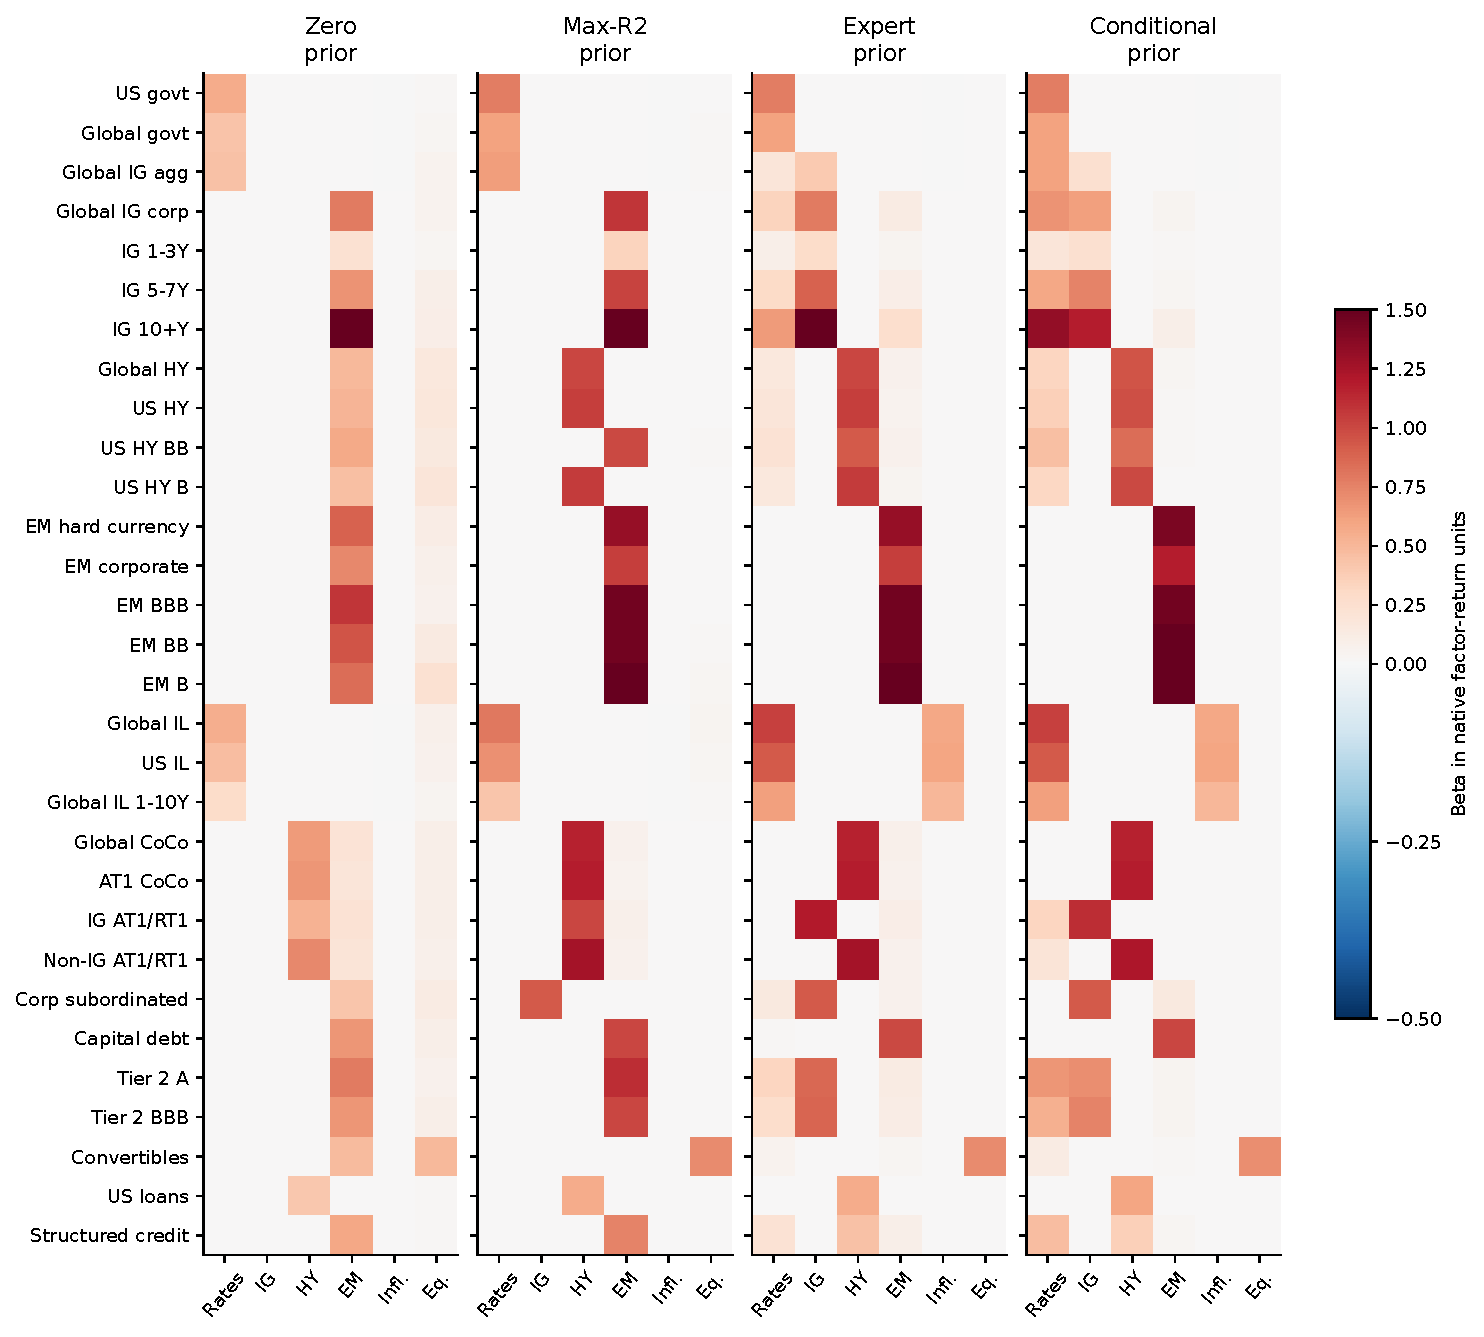
\includegraphics[width=.94\linewidth]{figures/fi_loadings.pdf}
\caption{Endpoint loadings for all thirty indices. Panels share the same factor units and colour scale. Colour saturation clips at -0.5 and 1.5 for legibility; full numerical coefficients are retained in the evidence files. Differences are complete-policy effects, including prior-informed signs.}
\end{figure}

\subsection{Independent duration evidence and hybrid limitations}

Option-adjusted duration was withheld from target construction. Thirteen panel indices have a usable observation at or before the cutoff in the saved duration panels. Table 2 reports the pooled rank association. It does not favour Conditional prior. That adverse result limits any claim that conditioned targets have already been validated as a physical duration model.

\begin{table}[pos=htbp]
\centering
\small
\caption{Independent descriptive association between Rates beta and available option-adjusted duration.}
\begin{adjustbox}{max width=\linewidth}
\begin{tabular}{lrr}
\toprule
Policy & Paired observations & Spearman: Rates / OAD \\
\midrule
Zero prior & 13 & +0.566 \\
Max-R2 prior & 13 & -0.154 \\
Expert prior & 13 & +0.236 \\
Conditional prior & 13 & +0.198 \\
\bottomrule
\end{tabular}
\end{adjustbox}
\end{table}

OAD is in years, whereas the Rates factor is a scaled return series. A single cross-sectional correlation mixes maturity, optionality, issuer mix and factor units. The maturity-bucket observations are also retained individually in the supplement. Without verified factor DV01, neither beta nor this rank association is a calibrated duration estimate. The evidence supports improved attribution as a working interpretation that still needs independent sensitivity checks.

Convertible Equity remains eligible in every main arm. Broad CoCos and flexible credit funds retain automatic fallback when classification is unclear. The supplementary three-factor and rating-based cases expose sensitivity to mapping assumptions; they are not allowed to redefine the primary arms after outcomes are known. The full twelve-factor coefficient and CMA records retain unfavourable cases as well as the motivating examples.

\subsection{Prior centre, signs and shared penalties}

\begin{table}[pos=htbp]
\centering
\small
\caption{Thirty-index two-by-two control: zero or conditioned centre, with detected or prior-informed solver signs. Hard restrictions and clustering remain fixed.}
\begin{adjustbox}{max width=\linewidth}
\begin{tabular}{lrrr}
\toprule
Centre / sign layer & Mean fit R2 \% & Global IL Inflation & IG aggregate R2 \% \\
\midrule
Zero prior / detected & 68.63 & 0.000 & 86.56 \\
Conditional prior / detected & 70.32 & 0.000 & 92.99 \\
Zero prior / prior & 68.63 & 0.000 & 86.56 \\
Conditional prior / prior & 73.62 & 0.581 & 92.99 \\
\bottomrule
\end{tabular}
\end{adjustbox}
\end{table}

The sign control holds the solver-facing matrix fixed within each centre comparison. At penalty zero, the two centres give identical predictions only under the same constraints and preprocessing; this invariance is verified. It would be incorrect to require identical fits when the prior also changes the feasible sign set. The separable-LASSO diagnostic removes cross-asset penalty coupling and is reported separately in the supplement.

\begin{table}[pos=htbp]
\centering
\small
\caption{IL-only intervention in the full CMA universe's monthly block. All non-IL priors and signs are identical; cluster labels are fixed. The CMA column is the direct beta-times-premium component only.}
\begin{adjustbox}{max width=\linewidth}
\begin{tabular}{lrrr}
\toprule
Full monthly block & Univariate IL fit \% & Joint IL fit \% & Direct factor CMA change, bp \\
\midrule
Global IL & 66.89 & 83.62 & +62.7 \\
Global IG agg & 87.86 & 82.58 & -7.3 \\
Global IG corp & 83.06 & 83.06 & 0.0 \\
Global HY & 76.87 & 76.87 & +0.0 \\
EM hard currency & 85.94 & 85.94 & 0.0 \\
\bottomrule
\end{tabular}
\end{adjustbox}
\end{table}

Changing IL targets improves IL reconstruction but reduces the IG aggregate's fitted R-squared. Its own prior and sign settings do not change. FCGL penalises a cluster's deviations jointly for each factor, so changing one member's target alters the shared penalty's marginal cost for its neighbours. The current-calibration replay reproduces the saved full-universe model to numerical precision; both IL intervention arms use the same per-response loss normalization, fixed monthly penalty and revised sign analytics. Quarterly and cash blocks do not share the monthly penalty and need no intervention. The thirty-index panel therefore cannot be expected to reproduce full-universe coefficients merely by matching per-asset settings.

\section{Consequences for capital market assumptions}

All policies use the same approved 2026 MATF-CMA premium vector, cash rate, currency treatment and factor covariance. The IG, HY and EM blended annual factor premia are 1.6831\%, 2.3669\% and 1.9829\%. They retain the disclosed first-order 1x tracker credit-notional/NAV convention and verified MATF scaling. The strategic spread and credit-loss inputs are policy calibrations, not independently benchmark-estimated actuarial quantities. The EM annual default-loss assumption is 15 bp (0.30\% default probability and 50\% loss given default). The long-run premium translates the strategic spread/loss scenario using current factor exposure. These inputs are fixed across prior policies.

For an asset with fixed external assumptions, the comparison is

\begin{equation}
\mu_i=r_f+\beta_i^{\mathsf T}\pi+A_i,\qquad
\Delta\mu_i=(\Delta\beta_i)^{\mathsf T}\pi+\Delta A_i.
\end{equation}

All eighteen CMA-source rows admit zero residual alpha. The broader MATF-CMA baseline retains PE 50\% and ILS 100\% alpha admission; neither enters this fixed-income panel. Their existing regional Rates adjustment is retained. Its load multiplier is fixed to the baseline so changes isolate the loading specification; its remaining beta dependence is shown separately. The twelve additional indices have illustrative zero-alpha CMAs with no regional overlay. They are not newly approved official CMA rows. Fund results assess fit and attribution without introducing a fund-alpha policy. Section 9.3 compares historical stress losses implied by the same endpoint loadings.

\begin{table}[pos=htbp]
\centering
\small
\caption{Annual arithmetic total-return CMAs and implied model volatility for the selected index cases. These are specification sensitivities, not revised distributed assumptions.}
\begin{adjustbox}{max width=\linewidth}
\begin{tabular}{lrrrrrr}
\toprule
Index & \shortstack{Zero\\prior} \% & \shortstack{Max-R2\\prior} \% & \shortstack{Expert\\prior} \% & \shortstack{Conditional\\prior} \% & \shortstack{Conditional minus\\Max-R2, bp} & \shortstack{Conditional\\prior} vol \% \\
\midrule
Global IG agg & 4.80 & 4.90 & 5.02 & 5.20 & +29.8 & 3.85 \\
Global IG corp & 5.94 & 6.30 & 6.06 & 5.97 & -33.6 & 5.52 \\
Global HY & 5.78 & 6.57 & 6.83 & 6.77 & +20.2 & 5.54 \\
EM hard currency & 6.34 & 6.80 & 6.77 & 6.98 & +18.2 & 7.02 \\
Global IL & 5.01 & 5.13 & 5.61 & 5.61 & +47.8 & 5.73 \\
Convertibles & 7.00 & 6.89 & 6.99 & 6.98 & +9.6 & 12.22 \\
\bottomrule
\end{tabular}
\end{adjustbox}
\end{table}

\begin{figure}[pos=htbp]
\centering
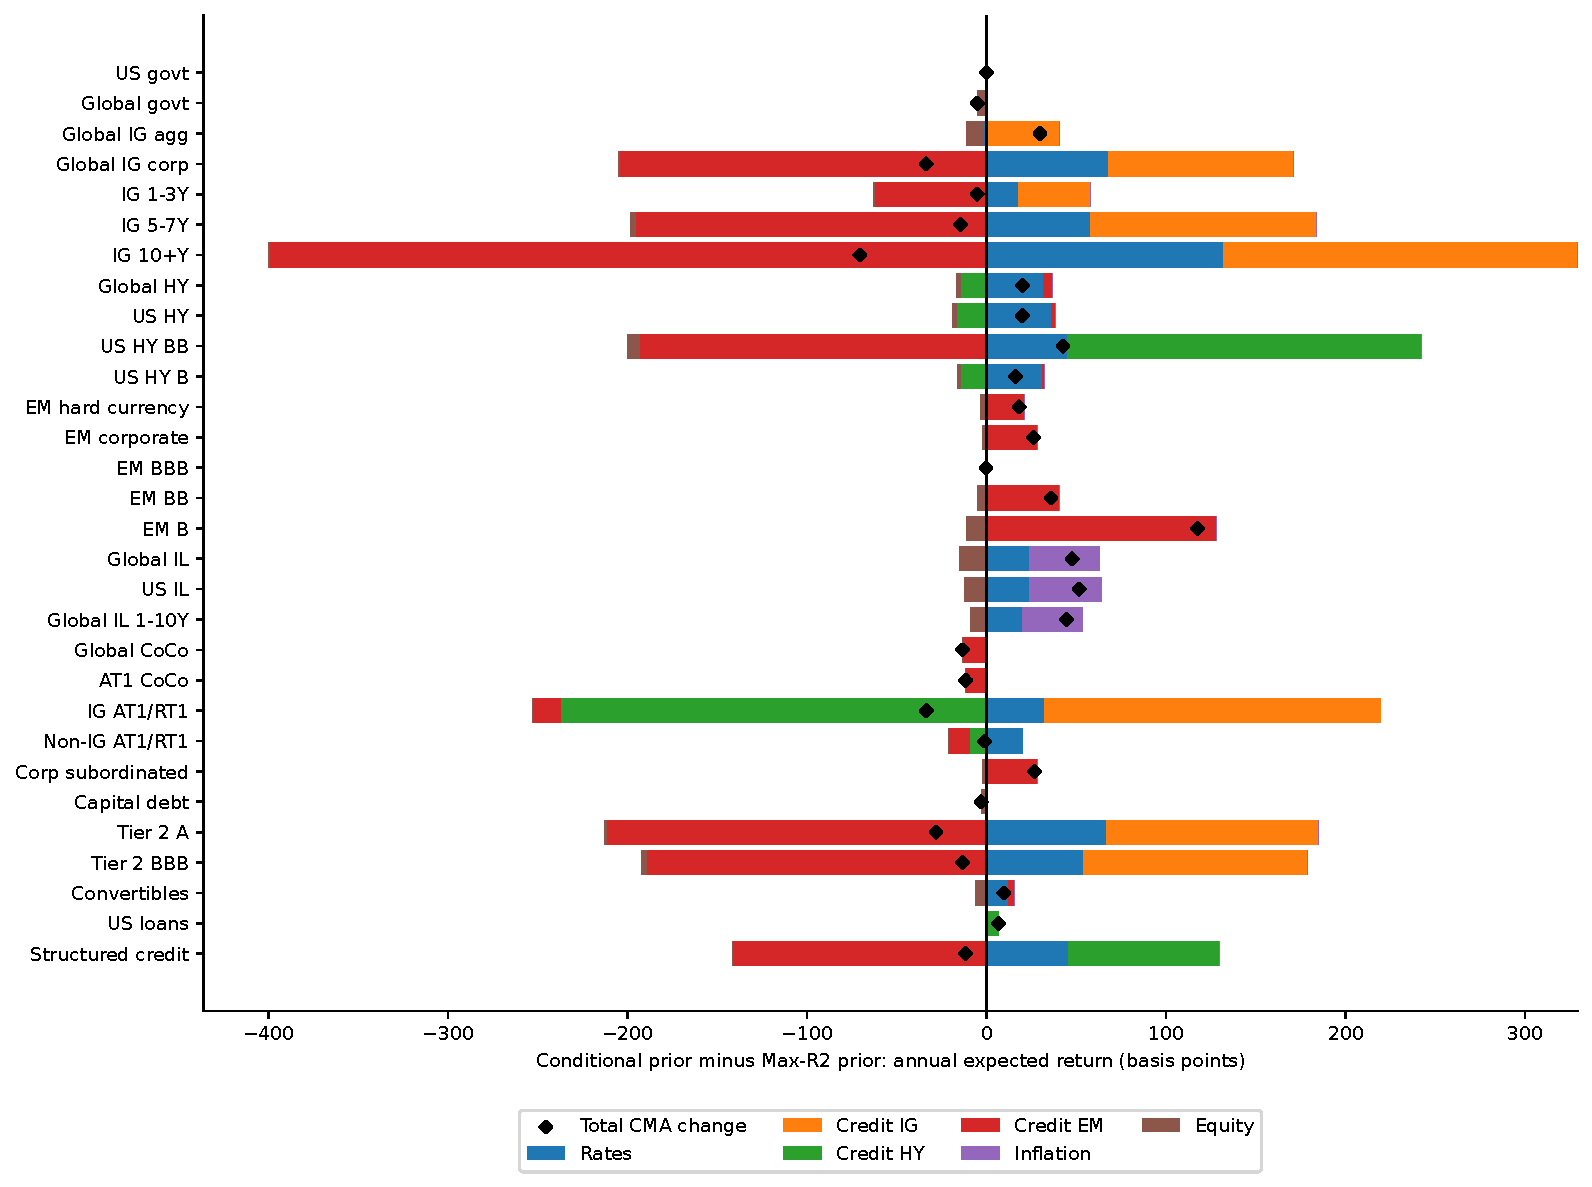
\includegraphics[width=.94\linewidth]{figures/fi_cma.pdf}
\caption{Conditional prior minus Max-R2 prior CMA sensitivity across thirty indices. Bars show six factor contributions; diamonds show total change, including the other six factors and any regional Rates adjustment. All external premia and alpha admissions are fixed.}
\end{figure}

\begin{table}[pos=htbp]
\centering
\small
\caption{Fixed illustrative bond portfolio: equal weights across seven index categories, then equal weights within category. Volatility uses the fixed factor covariance plus each fit's residual variances.}
\begin{adjustbox}{max width=\linewidth}
\begin{tabular}{lrrrrr}
\toprule
Policy & Total CMA \% & Excess CMA \% & Model vol \% & Sharpe (rf=0) & Excess Sharpe \\
\midrule
Zero prior & 5.60 & 1.42 & 3.53 & 1.59 & 0.40 \\
Max-R2 prior & 5.94 & 1.76 & 3.91 & 1.52 & 0.45 \\
Expert prior & 6.02 & 1.84 & 3.98 & 1.51 & 0.46 \\
Conditional prior & 6.05 & 1.87 & 4.30 & 1.41 & 0.44 \\
\bottomrule
\end{tabular}
\end{adjustbox}
\end{table}

The Table 6 portfolio weights do not respond to the model and are not optimised. A separate appendix exhibit uses the Table 12 CMAs to trace the systematic-risk efficient frontier. Factor covariance is held fixed, but changing loadings and residual variance changes implied risk. This is distinct from the unchanged realised volatility of the underlying return series. Total-return Sharpe divides the total arithmetic CMA by model volatility with rf=0; excess Sharpe subtracts cash in the numerator. Neither ratio measures realised strategy performance.

Every asset CMA reconciles independently to the owner calculation, including the permitted regional adjustment. The supplement scales the three credit premia together by 0.8, 1.0 and 1.2 while retaining other inputs. This addresses the stated tracker-unit approximation; it does not establish that the approximation is exact. Substituting a correlated return proxy can have an expected-return effect even when its prediction effect is small.

\section{Next-quarter explanation and transfer to funds}

At each quarter end, all targets, automatic signs, training means and clusters are re-estimated using past observations. Beta and the training economic intercept are frozen for the following three months. Predictions use contemporaneously realised factors. The score pools squared errors across the scored history before computing

\begin{equation}
R^2_{\rm OOS}=1-\frac{\sum_t(y_{it}-\widehat\alpha_{i,t-1}-x_t^{\mathsf T}\widehat\beta_{i,t-1})^2}
{\sum_t(y_{it}-\overline y_{i,t-1})^2}.
\end{equation}

The benchmark mean is the same past-only span-60 weighted mean for both estimation spans. We do not average three-month R-squared values. Negative asset scores remain in the tables. Future-input mutation tests at the first, middle and last calibration dates leave every arm's fitted coefficients unchanged. This verifies the study's truncation boundary, not the historical-vintage factor-construction issue described above.

\begin{table}[pos=htbp]
\centering
\small
\caption{Arithmetic average of per-asset pooled held-out R-squared, including eligible later entrants. Each asset is weighted equally in this descriptive table.}
\begin{adjustbox}{max width=\linewidth}
\begin{tabular}{lrrrrrr}
\toprule
Panel & Span & Assets & \shortstack{Zero\\prior} \% & \shortstack{Max-R2\\prior} \% & \shortstack{Expert\\prior} \% & \shortstack{Conditional\\prior} \% \\
\midrule
Indices & 60 & 30 & 58.26 & 62.73 & 65.45 & 69.39 \\
Indices & 36 & 30 & 56.57 & 60.74 & 65.43 & 69.36 \\
Funds & 60 & 12 & 61.23 & 66.31 & 71.15 & 73.59 \\
Funds & 36 & 12 & 62.26 & 64.30 & 70.48 & 73.36 \\
\bottomrule
\end{tabular}
\end{adjustbox}
\end{table}

At the specified penalty, Conditional prior has the highest panel average for both spans and both panels. Expert prior is not uniformly superior to Max-R2 prior, and Conditional prior does not win for every asset. The span-36 results retain the ordering but should not be selected simply because a relative gain looks larger. Absolute scores, coefficient movement and a common benchmark denominator must be considered together.

\begin{figure}[pos=htbp]
\centering
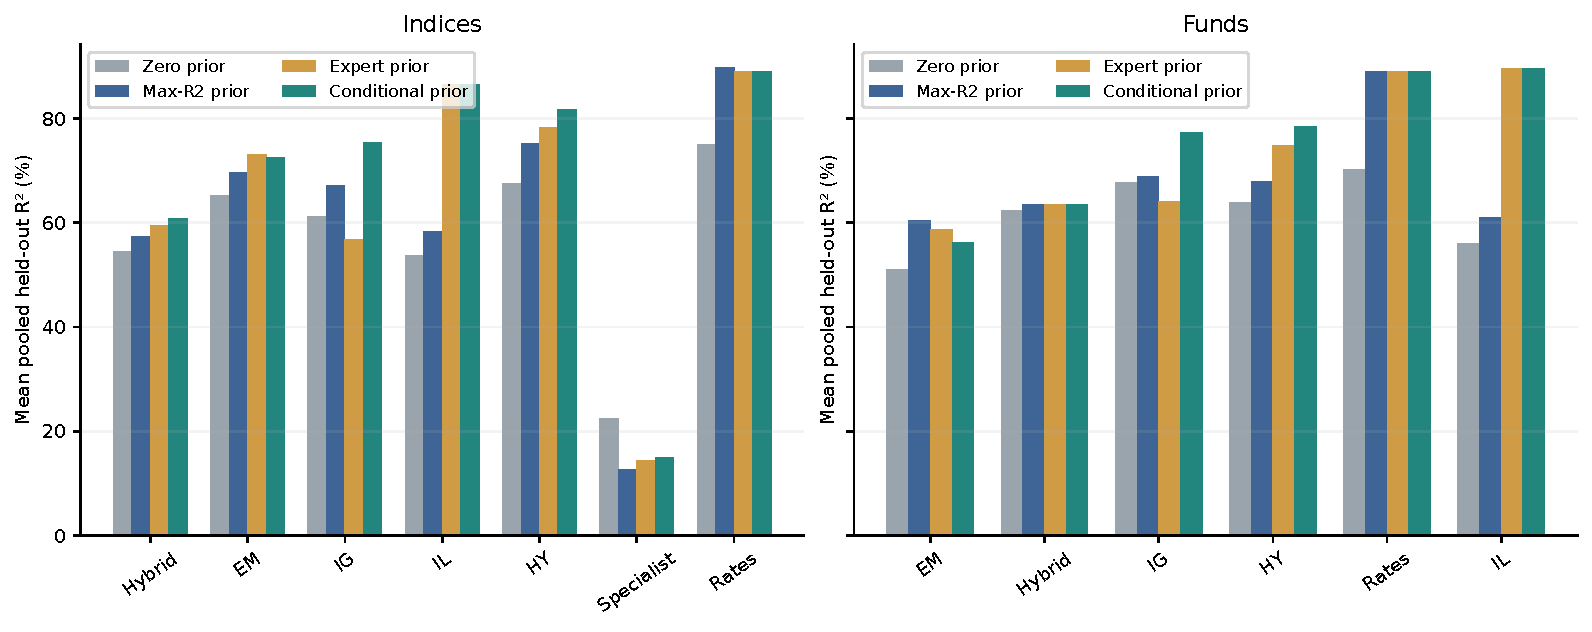
\includegraphics[width=.94\linewidth]{figures/fi_oos.pdf}
\caption{Mean pooled held-out R-squared by category at span 60. Rates controls are shown separately. Counts and active/passive splits are in the appendix; related indices share underlying risks and are not independent trials.}
\end{figure}

For exploratory uncertainty we use only the fixed initial non-Rates cohort: twenty-seven indices and ten funds. Assets are averaged within category, then categories receive equal weight. Entire paired calendar quarters are resampled jointly across arms and assets using the QIS circular stationary bootstrap, with 5,000 samples and a mean block of four quarters \citep{politis1994}. Two- and eight-quarter block sensitivities are retained. These are different estimands from the all-asset averages in Table 7.

\begin{table}[pos=htbp]
\centering
\small
\caption{Category-balanced paired gains in held-out R-squared at span 60. Intervals are exploratory percentile intervals, in percentage points.}
\begin{adjustbox}{max width=\linewidth}
\begin{tabular}{lrrrr}
\toprule
Panel & Cohort & Contrast & Gain, pp & 95\% block interval, pp \\
\midrule
Indices & 27 & Max-R2 prior minus Zero prior & +3.60 & [-3.09, +7.42] \\
Indices & 27 & Expert prior minus Max-R2 prior & +4.77 & [-1.78, +10.47] \\
Indices & 27 & Conditional prior minus Max-R2 prior & +10.75 & [+2.77, +17.92] \\
Indices & 27 & Conditional prior minus Zero prior & +14.35 & [+1.19, +24.87] \\
Funds & 10 & Max-R2 prior minus Zero prior & +4.53 & [-1.54, +7.10] \\
Funds & 10 & Expert prior minus Max-R2 prior & +5.99 & [+0.62, +12.28] \\
Funds & 10 & Conditional prior minus Max-R2 prior & +8.97 & [+2.74, +16.08] \\
Funds & 10 & Conditional prior minus Zero prior & +13.50 & [+2.53, +22.25] \\
\bottomrule
\end{tabular}
\end{adjustbox}
\end{table}

Conditional prior's gain over Max-R2 prior is positive across the main interval for both panels in the revised run. The separate zero-penalty controls nevertheless prevent attributing every gain to the FCGL penalty. A short, nonstationary period containing the pandemic, the 2022 bond drawdown and subsequent recovery does not provide a general coverage guarantee. The 2020, 2022 and 2023 episode scores are retained as diagnostics, not independent experiments.

\begin{table}[pos=htbp]
\centering
\small
\caption{Mean absolute quarterly change per factor coefficient at span 60. Native beta units; all twelve factors included.}
\begin{adjustbox}{max width=\linewidth}
\begin{tabular}{lrrrr}
\toprule
Panel & \shortstack{Zero\\prior} & \shortstack{Max-R2\\prior} & \shortstack{Expert\\prior} & \shortstack{Conditional\\prior} \\
\midrule
Indices & 0.0166 & 0.0180 & 0.0113 & 0.0084 \\
Funds & 0.0165 & 0.0155 & 0.0132 & 0.0109 \\
\bottomrule
\end{tabular}
\end{adjustbox}
\end{table}

The smaller coefficient movement under Conditional prior is useful operationally, but some of it can result from persistent targets. It is not proof that the underlying exposures are stable. The evidence bundle additionally records automatic-winner switches, sign switches, per-asset RMSE and residual bias. Isolated-factor scenario changes are obtained by multiplying coefficient changes by a stated factor return shock.

\begin{figure}[pos=htbp]
\centering
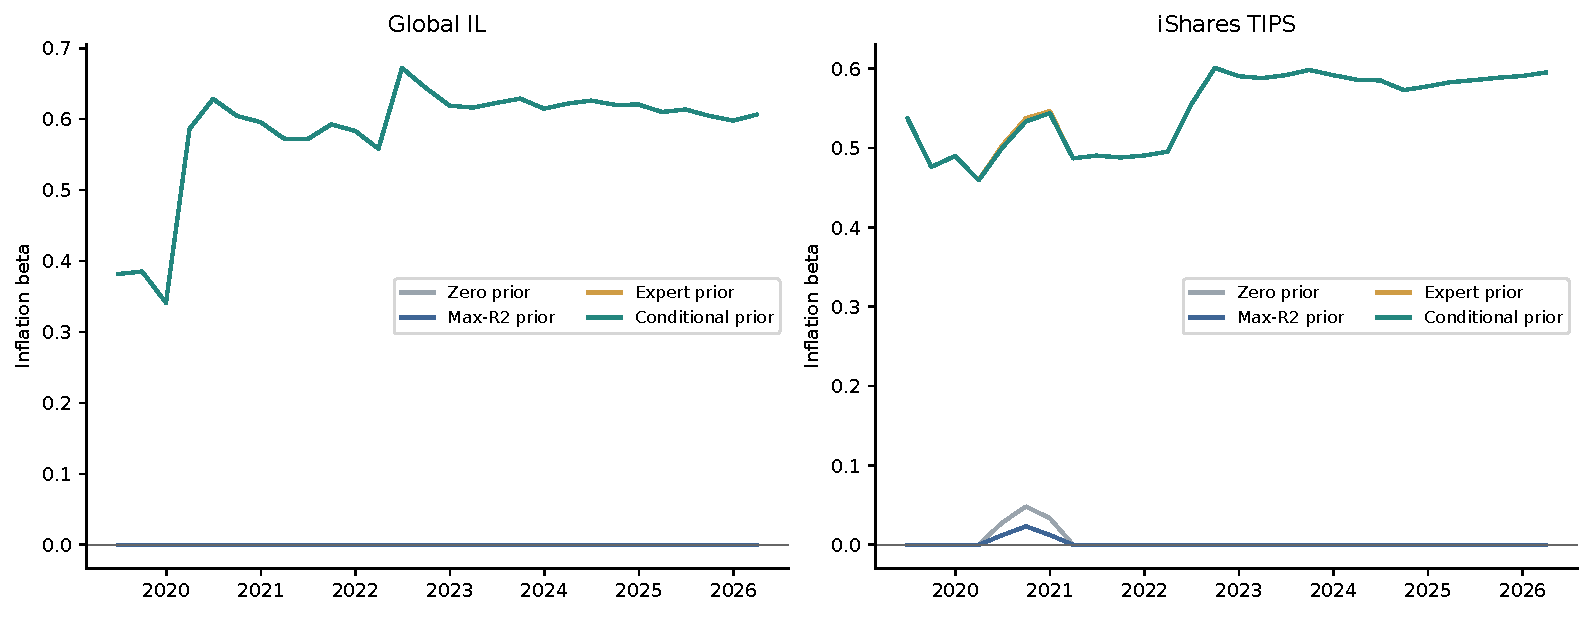
\includegraphics[width=.94\linewidth]{figures/fi_il_path.pdf}
\caption{Quarterly Inflation coefficients for Global IL and iShares TIPS at span 60. The mapped policies use the same Rates/Inflation prior for IL; small differences can arise from their other assets' targets through the shared penalty.}
\end{figure}

\section{Supporting known-truth experiments}

Two simulation families separate known loading truth from empirical interpretation. The first generates government, IG, HY, EM and convertible responses under low or high credit-factor correlation, a deliberately wrong IG-to-EM mapping, and an omitted Equity factor. The second generates a Rates/Inflation response whose marginal Inflation sign differs from its conditional sign, plus a weak negative Inflation exposure. Neighbouring IG assets allow an IL-only shared-penalty intervention. True coefficients are fixed design choices, not empirical Conditional prior estimates.

Each design has sixty- and 120-month training samples, 240 independent test months, and 200 paired replications. A separate five-replication pilot is excluded. All estimated policies share the draws, penalty, sign rules and cluster labels within a replication; their target magnitudes are estimated from training data. The oracle uses the true soft target and is explicitly given additional information. In the omitted-factor design Equity is unavailable to every fitted model, including the oracle; omitted loadings are treated as zero when errors are measured.

\begin{table}[pos=htbp]
\centering
\small
\caption{Monte Carlo mean absolute annual CMA error in basis points, averaged across six synthetic assets. MCSE uses independent replications, not individual assets.}
\begin{adjustbox}{max width=\linewidth}
\begin{tabular}{lrrrrrrr}
\toprule
Design & Months & \shortstack{Zero\\prior} & \shortstack{Max-R2\\prior} & \shortstack{Expert\\prior} & \shortstack{Conditional\\prior} & Oracle & \shortstack{Conditional\\prior} MCSE \\
\midrule
Credit high & 60 & 39.6 & 30.3 & 14.6 & 5.9 & 0.1 & 0.2 \\
Credit high & 120 & 43.5 & 33.6 & 14.9 & 5.8 & 0.0 & 0.2 \\
Credit low & 60 & 44.5 & 36.1 & 15.3 & 6.8 & 0.1 & 0.2 \\
Credit low & 120 & 50.2 & 39.9 & 16.4 & 7.0 & 0.0 & 0.1 \\
Credit omitted & 60 & 61.5 & 51.5 & 33.5 & 24.4 & 25.2 & 0.4 \\
Credit omitted & 120 & 66.8 & 55.4 & 35.1 & 24.5 & 26.3 & 0.4 \\
Credit wrong & 60 & 40.3 & 30.9 & 16.3 & 7.2 & 0.1 & 0.2 \\
Credit wrong & 120 & 43.3 & 33.2 & 16.3 & 6.8 & 0.0 & 0.2 \\
IL sign & 60 & 40.1 & 31.0 & 14.5 & 6.0 & 0.1 & 0.1 \\
IL sign & 120 & 44.0 & 34.0 & 15.3 & 6.1 & 0.0 & 0.1 \\
IL weak & 60 & 28.3 & 24.7 & 21.1 & 15.3 & 6.1 & 0.4 \\
IL weak & 120 & 27.1 & 23.3 & 18.9 & 13.0 & 2.3 & 0.3 \\
\bottomrule
\end{tabular}
\end{adjustbox}
\end{table}

\begin{figure}[pos=htbp]
\centering
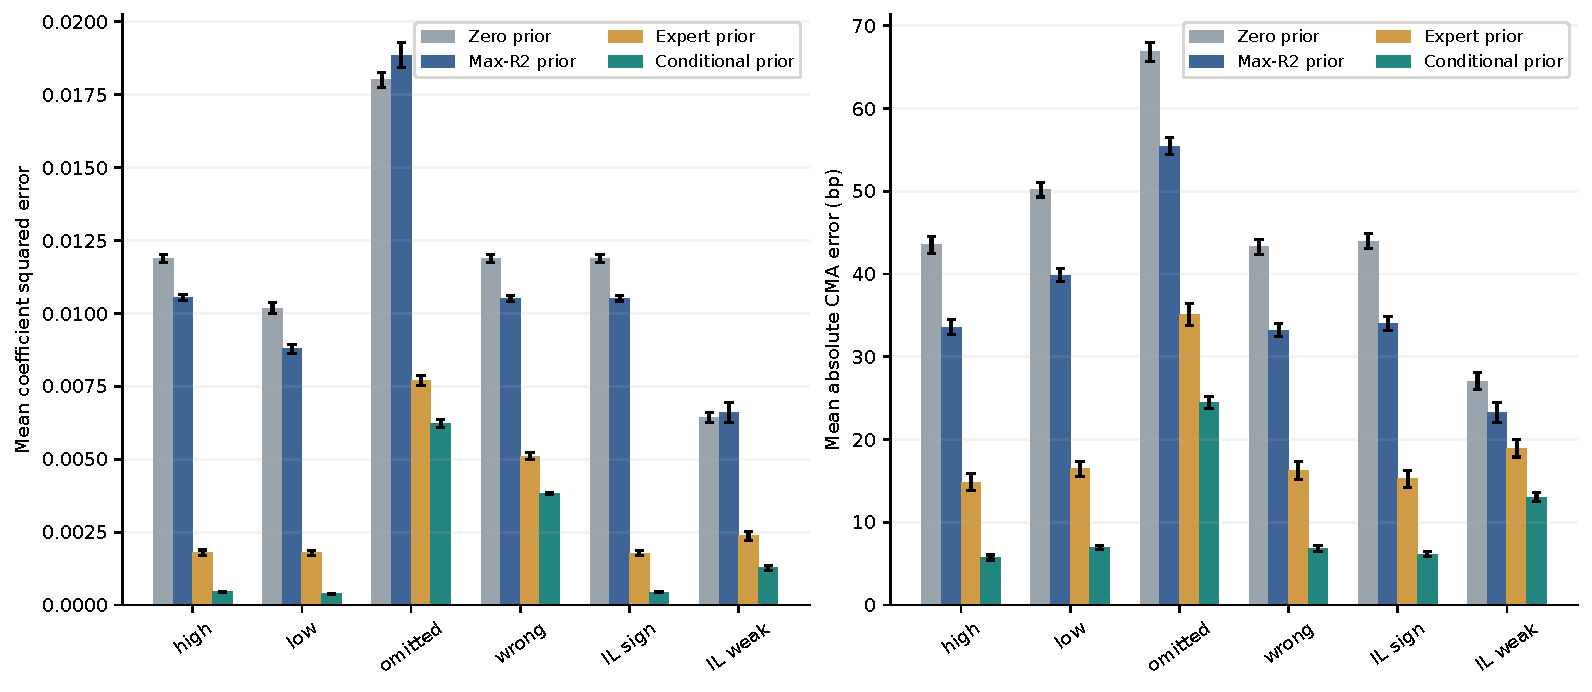
\includegraphics[width=.94\linewidth]{figures/fi_mc.pdf}
\caption{Coefficient and CMA errors with 120 training months. Error bars are 1.96 Monte Carlo standard errors of the estimated mean, not empirical confidence intervals for an investment forecast. The deliberately wrong and omitted-factor cases remain in the comparison.}
\end{figure}

\begin{table}[pos=htbp]
\centering
\small
\caption{Focal Monte Carlo diagnostics with 120 training months: mean absolute CMA error, in basis points, for the directly affected asset. Cross-asset averages can conceal these losses.}
\begin{adjustbox}{max width=\linewidth}
\begin{tabular}{lrrrrr}
\toprule
Design & Affected asset & \shortstack{Zero\\prior} & \shortstack{Max-R2\\prior} & \shortstack{Expert\\prior} & \shortstack{Conditional\\prior} \\
\midrule
high & IG & 39.2 & 30.0 & 17.3 & 3.8 \\
wrong & IG & 39.0 & 29.7 & 25.1 & 10.7 \\
omitted & Convertible & 175.4 & 152.7 & 145.5 & 129.4 \\
IL weak & IL & 8.1 & 15.7 & 13.9 & 13.6 \\
\bottomrule
\end{tabular}
\end{adjustbox}
\end{table}

The deliberately wrong IG-to-EM mapping increases IG loading error: mean beta MSE is 0.0204, against 0.0147 for automatic selection. Yet its mean absolute CMA error is lower at the current premium calibration (10.7 versus 29.7 bp). The smaller IG/EM premium gap and compensating loading errors can hide incorrect economic attribution; a small CMA error does not validate the mapping. Omitting Equity leaves a large convertible error that even the restricted oracle cannot repair. For the weak negative IL exposure, the estimated joint target sometimes has the wrong sign and its CMA error exceeds the zero-target control. These cases show why a higher panel-average score cannot validate every mapping.

The simulation is a mechanism check with synthetic monthly factor scales. It cannot identify true betas in the licensed histories or establish universal dominance. The supplement also reports conditional prediction error, raw sign alignment, false credit exposures on the government control, scenario error and IL spillovers. Raw sign alignment includes small solver coefficients and must be distinguished from materially recovered exposure. Every draw is retained; solver failures would stop the run rather than disappear from the averages. Weighted target slopes, predictions and CMA errors are checked independently.

Two small offline examples demonstrate IG/EM proxy confusion and the conditional Inflation sign using only the public FactorLasso API. Their portable default is the open-source CLARABEL solver; this private run explicitly selects MOSEK. They generate synthetic data locally and do not claim to reproduce MATF returns. They make the proposed policy inspectable without a market-data subscription.

\section{A practical selection and review rule}

For ordinary IG, HY and hard-currency EM indices, use the mandate to nominate a credit factor, then assess a joint Rates/credit target against the automatic and zero-target controls. For IL, estimate Rates and Inflation jointly and allow the estimated prior direction to override automatic detection only where no explicit hard rule forbids it. For convertibles, keep Equity eligible and inspect the cost of omitting it. For ambiguous hybrids, mixed-credit mandates or insufficient classification, retain automatic selection and flag the missing economic information.

Before adopting a mapping, review its raw/effective target, sign overrides, residual diagnostics, held-out behaviour, independent sensitivities and CMA contribution. Refit the full affected estimation block: an isolated asset test cannot reveal shared-penalty spillovers. A mapping change that improves one sleeve can harm another. Retain the old specification as a comparison and record any hard-rule conflict rather than silently treating the requested prior as effective.

The evidence supports Rates-conditioned mapping as the leading candidate for further controlled use, with automatic fallback. It does not justify replacing every automatic target, asserting a physical DV01 interpretation of raw beta, or selecting a method because its CMA is higher. Independent duration evidence is mixed; fund uncertainty is wider; wrong expert information remains costly. The prior-policy comparisons hold universe worksheets and expected-return inputs fixed.

\section{Analytical support and limitations}

For a centred linear response $y=\sum_k\beta_k x_k+\varepsilon$, an exogenous-error marginal OLS slope satisfies

\begin{equation}
b_j^{\rm marginal}=\beta_j+\sum_{k\ne j}\beta_k\frac{\operatorname{Cov}(x_j,x_k)}{\operatorname{Var}(x_j)}.
\end{equation}

A marginal winner can absorb Rates or correlated credit exposures. Joint weighted OLS on selected factors removes the contributions of the other selected factors; it does not remove omitted-variable effects. In the two-factor IL case, a sufficiently negative Rates/Inflation covariance can make the marginal Inflation slope negative even when its conditional coefficient is positive. The simulation's stronger IL case has Rates beta 0.9, Inflation beta 0.45, equal factor scales and correlation -0.8, implying a population marginal Inflation slope of -0.27.

For two standardized correlated factors, an attribution error $(a,-a)$ has prediction variance $2a^2(1-\rho)$. As correlation approaches one, materially different allocations can produce similar predictions. Their CMA difference is $a(\pi_1-\pi_2)$, which need not shrink with correlation. These identities explain why prediction and economic attribution require separate checks.

Prior-centred shrinkage regularises deviations from the target. Classical zero-centred LASSO \citep{tibshirani1996}, proxy-based transfer \citep{bastani2021}, transfer penalties \citep{takada2020}, and pretraining \citep{craig2026} motivate different uses of prior information; their guarantees are not imported into this same-sample target policy. Univariate-guided regression \citep{chatterjee2025} uses a different staged estimator. Relaxed LASSO \citep{meinshausen2007}, fundamental beta priors \citep{cosemans2016}, and covariance shrinkage \citep{ledoit2003} address related but distinct problems.

The main limitations are fixed-vintage histories, overlapping benchmarks, a previously inspected sample, a fixed rather than separately tuned penalty, incomplete independent sensitivity data, and the disclosed credit-factor notional approximation. Mandate labels can be wrong or incomplete. A positive conditional Inflation beta is not a guarantee of protection against every inflation event. Better next-quarter explanation does not establish superior long-horizon expected-return forecasts. Earlier versions of this note used different factor/sign specifications and fixed numerical targets; their scores are archived rather than pooled with the present study.

\FloatBarrier\section{Appendix: complete compact results}

\begin{table}[pos=htbp]
\centering
\small
\setlength{\tabcolsep}{3pt}
\caption{Thirty-index conditioned estimates (Conditional prior), held-out Conditional prior minus Max-R2 prior gains at span 60, annual arithmetic total CMA, and annual systematic MATF volatility (Factor vol). Bloomberg identifiers omit the common Index suffix. CMA-source rows retain their frozen policy; twelve additional benchmark rows are illustrative zero-alpha calculations. Factor volatility excludes residual risk; Tables 5 and 6 include it. Full names, source and mapping status are in the roster file.}
\begin{adjustbox}{max width=\linewidth}
\begin{tabular}{llrrrrrrrrr}
\toprule
Short name & Bloomberg & Rates & IG & HY & EM & Infl. & Equity & OOS gain, pp & CMA \% & Factor vol \% \\
\midrule
US govt & LUATTRUU & \cellcolor[HTML]{E37E64}\textcolor{black}{0.770} & \cellcolor[HTML]{FFFFFF}\textcolor{black}{0.000} & \cellcolor[HTML]{FFFFFF}\textcolor{black}{0.000} & \cellcolor[HTML]{FFFFFF}\textcolor{black}{0.000} & \cellcolor[HTML]{FFFFFF}\textcolor{black}{0.000} & \cellcolor[HTML]{FFFFFF}\textcolor{black}{0.000} & +0.0 & 4.96 & 4.36 \\
Global govt & LGTRTRUH & \cellcolor[HTML]{F3A481}\textcolor{black}{0.604} & \cellcolor[HTML]{FFFFFF}\textcolor{black}{0.000} & \cellcolor[HTML]{FFFFFF}\textcolor{black}{0.000} & \cellcolor[HTML]{FFFFFF}\textcolor{black}{0.000} & \cellcolor[HTML]{FFFFFF}\textcolor{black}{0.000} & \cellcolor[HTML]{FFFFFF}\textcolor{black}{0.000} & -1.4 & 4.79 & 3.42 \\
Global IG agg & LEGATRUH & \cellcolor[HTML]{F3A481}\textcolor{black}{0.606} & \cellcolor[HTML]{FCE0D0}\textcolor{black}{0.243} & \cellcolor[HTML]{FFFFFF}\textcolor{black}{0.000} & \cellcolor[HTML]{FFFFFF}\textcolor{black}{0.000} & \cellcolor[HTML]{FFFFFF}\textcolor{black}{0.000} & \cellcolor[HTML]{FFFFFF}\textcolor{black}{0.000} & +3.9 & 5.20 & 3.71 \\
Global IG corp & LGCPTRUH & \cellcolor[HTML]{EC9374}\textcolor{black}{0.677} & \cellcolor[HTML]{F2A17F}\textcolor{black}{0.613} & \cellcolor[HTML]{FFFFFF}\textcolor{black}{0.000} & \cellcolor[HTML]{F8F3F0}\textcolor{black}{0.038} & \cellcolor[HTML]{FFFFFF}\textcolor{black}{0.000} & \cellcolor[HTML]{FFFFFF}\textcolor{black}{0.000} & +12.3 & 5.97 & 5.16 \\
IG 1-3Y & H09627US & \cellcolor[HTML]{FBE6DA}\textcolor{black}{0.179} & \cellcolor[HTML]{FCE0D0}\textcolor{black}{0.237} & \cellcolor[HTML]{FFFFFF}\textcolor{black}{0.000} & \cellcolor[HTML]{F7F5F4}\textcolor{black}{0.014} & \cellcolor[HTML]{FFFFFF}\textcolor{black}{0.000} & \cellcolor[HTML]{FFFFFF}\textcolor{black}{0.000} & +5.4 & 4.79 & 1.63 \\
IG 5-7Y & H09629US & \cellcolor[HTML]{F5A886}\textcolor{black}{0.579} & \cellcolor[HTML]{E58368}\textcolor{black}{0.747} & \cellcolor[HTML]{FFFFFF}\textcolor{black}{0.000} & \cellcolor[HTML]{F8F4F2}\textcolor{black}{0.029} & \cellcolor[HTML]{FFFFFF}\textcolor{black}{0.000} & \cellcolor[HTML]{FFFFFF}\textcolor{black}{0.000} & +10.4 & 6.08 & 5.15 \\
IG 10+Y & H09631US & \cellcolor[HTML]{930E26}\textcolor{white}{1.313} & \cellcolor[HTML]{B41C2D}\textcolor{white}{1.173} & \cellcolor[HTML]{FFFFFF}\textcolor{black}{0.000} & \cellcolor[HTML]{F9EFE9}\textcolor{black}{0.087} & \cellcolor[HTML]{FFFFFF}\textcolor{black}{0.000} & \cellcolor[HTML]{FFFFFF}\textcolor{black}{0.000} & +9.3 & 7.65 & 10.00 \\
Global HY & H23059US & \cellcolor[HTML]{FCD7C2}\textcolor{black}{0.318} & \cellcolor[HTML]{FFFFFF}\textcolor{black}{0.000} & \cellcolor[HTML]{D05548}\textcolor{white}{0.938} & \cellcolor[HTML]{F8F4F2}\textcolor{black}{0.025} & \cellcolor[HTML]{FFFFFF}\textcolor{black}{0.000} & \cellcolor[HTML]{FFFFFF}\textcolor{black}{0.000} & +3.4 & 6.77 & 4.95 \\
US HY & LF98TRUU & \cellcolor[HTML]{FBD0B9}\textcolor{black}{0.362} & \cellcolor[HTML]{FFFFFF}\textcolor{black}{0.000} & \cellcolor[HTML]{CE4F45}\textcolor{white}{0.963} & \cellcolor[HTML]{F7F5F4}\textcolor{black}{0.012} & \cellcolor[HTML]{FFFFFF}\textcolor{black}{0.000} & \cellcolor[HTML]{FFFFFF}\textcolor{black}{0.000} & +5.1 & 6.85 & 5.14 \\
US HY BB & I00182US & \cellcolor[HTML]{F8BFA4}\textcolor{black}{0.450} & \cellcolor[HTML]{FFFFFF}\textcolor{black}{0.000} & \cellcolor[HTML]{DC6E57}\textcolor{black}{0.833} & \cellcolor[HTML]{F7F5F4}\textcolor{black}{0.012} & \cellcolor[HTML]{FFFFFF}\textcolor{black}{0.000} & \cellcolor[HTML]{FFFFFF}\textcolor{black}{0.000} & +13.2 & 6.63 & 4.87 \\
US HY B & I00185US & \cellcolor[HTML]{FDD9C4}\textcolor{black}{0.314} & \cellcolor[HTML]{FFFFFF}\textcolor{black}{0.000} & \cellcolor[HTML]{CB4942}\textcolor{white}{0.991} & \cellcolor[HTML]{F7F6F6}\textcolor{black}{0.005} & \cellcolor[HTML]{FFFFFF}\textcolor{black}{0.000} & \cellcolor[HTML]{FFFFFF}\textcolor{black}{0.000} & +4.5 & 6.85 & 5.11 \\
EM hard currency & H04386US & \cellcolor[HTML]{FFFFFF}\textcolor{black}{0.000} & \cellcolor[HTML]{FFFFFF}\textcolor{black}{0.000} & \cellcolor[HTML]{FFFFFF}\textcolor{black}{0.000} & \cellcolor[HTML]{7C0722}\textcolor{white}{1.412} & \cellcolor[HTML]{FFFFFF}\textcolor{black}{0.000} & \cellcolor[HTML]{FFFFFF}\textcolor{black}{0.000} & +0.9 & 6.98 & 6.58 \\
EM corporate & JBCDCORE & \cellcolor[HTML]{FFFFFF}\textcolor{black}{0.000} & \cellcolor[HTML]{FFFFFF}\textcolor{black}{0.000} & \cellcolor[HTML]{FFFFFF}\textcolor{black}{0.000} & \cellcolor[HTML]{B41C2D}\textcolor{white}{1.181} & \cellcolor[HTML]{FFFFFF}\textcolor{black}{0.000} & \cellcolor[HTML]{FFFFFF}\textcolor{black}{0.000} & +9.0 & 6.52 & 5.51 \\
EM BBB & I12881US & \cellcolor[HTML]{F7F6F6}\textcolor{black}{0.001} & \cellcolor[HTML]{FFFFFF}\textcolor{black}{0.000} & \cellcolor[HTML]{FFFFFF}\textcolor{black}{0.000} & \cellcolor[HTML]{730421}\textcolor{white}{1.443} & \cellcolor[HTML]{FFFFFF}\textcolor{black}{0.000} & \cellcolor[HTML]{FFFFFF}\textcolor{black}{0.000} & -2.8 & 7.04 & 6.73 \\
EM BB & I05040US & \cellcolor[HTML]{FFFFFF}\textcolor{black}{0.000} & \cellcolor[HTML]{FFFFFF}\textcolor{black}{0.000} & \cellcolor[HTML]{FFFFFF}\textcolor{black}{0.000} & \cellcolor[HTML]{67001F}\textcolor{white}{1.648} & \cellcolor[HTML]{FFFFFF}\textcolor{black}{0.000} & \cellcolor[HTML]{FFFFFF}\textcolor{black}{0.000} & +4.0 & 7.45 & 7.69 \\
EM B & I05039US & \cellcolor[HTML]{FFFFFF}\textcolor{black}{0.000} & \cellcolor[HTML]{FFFFFF}\textcolor{black}{0.000} & \cellcolor[HTML]{FFFFFF}\textcolor{black}{0.000} & \cellcolor[HTML]{67001F}\textcolor{white}{2.153} & \cellcolor[HTML]{FFFFFF}\textcolor{black}{0.000} & \cellcolor[HTML]{FFFFFF}\textcolor{black}{0.000} & +2.6 & 8.45 & 10.04 \\
Global IL & LF94TRUH & \cellcolor[HTML]{C6413E}\textcolor{white}{1.030} & \cellcolor[HTML]{FFFFFF}\textcolor{black}{0.000} & \cellcolor[HTML]{FFFFFF}\textcolor{black}{0.000} & \cellcolor[HTML]{FFFFFF}\textcolor{black}{0.000} & \cellcolor[HTML]{F5A886}\textcolor{black}{0.581} & \cellcolor[HTML]{FFFFFF}\textcolor{black}{0.000} & +16.3 & 5.61 & 5.26 \\
US IL & LBUTTRUU & \cellcolor[HTML]{D35A4A}\textcolor{white}{0.923} & \cellcolor[HTML]{FFFFFF}\textcolor{black}{0.000} & \cellcolor[HTML]{FFFFFF}\textcolor{black}{0.000} & \cellcolor[HTML]{FFFFFF}\textcolor{black}{0.000} & \cellcolor[HTML]{F4A683}\textcolor{black}{0.593} & \cellcolor[HTML]{FFFFFF}\textcolor{black}{0.000} & +21.7 & 5.51 & 4.72 \\
Global IL 1-10Y & H21247US & \cellcolor[HTML]{F2A17F}\textcolor{black}{0.617} & \cellcolor[HTML]{FFFFFF}\textcolor{black}{0.000} & \cellcolor[HTML]{FFFFFF}\textcolor{black}{0.000} & \cellcolor[HTML]{FFFFFF}\textcolor{black}{0.000} & \cellcolor[HTML]{F7B799}\textcolor{black}{0.493} & \cellcolor[HTML]{FFFFFF}\textcolor{black}{0.000} & +46.8 & 5.13 & 3.23 \\
Global CoCo & H30902US & \cellcolor[HTML]{FFFFFF}\textcolor{black}{0.000} & \cellcolor[HTML]{FFFFFF}\textcolor{black}{0.000} & \cellcolor[HTML]{B72230}\textcolor{white}{1.156} & \cellcolor[HTML]{FFFFFF}\textcolor{black}{0.000} & \cellcolor[HTML]{FFFFFF}\textcolor{black}{0.000} & \cellcolor[HTML]{FFFFFF}\textcolor{black}{0.000} & -0.7 & 6.92 & 5.39 \\
AT1 CoCo & IBXXC1D3 & \cellcolor[HTML]{FFFFFF}\textcolor{black}{0.000} & \cellcolor[HTML]{FFFFFF}\textcolor{black}{0.000} & \cellcolor[HTML]{B41C2D}\textcolor{white}{1.183} & \cellcolor[HTML]{FFFFFF}\textcolor{black}{0.000} & \cellcolor[HTML]{FFFFFF}\textcolor{black}{0.000} & \cellcolor[HTML]{FFFFFF}\textcolor{black}{0.000} & -0.4 & 6.98 & 5.51 \\
IG AT1/RT1 & H30914US & \cellcolor[HTML]{FCD7C2}\textcolor{black}{0.323} & \cellcolor[HTML]{BD2D35}\textcolor{white}{1.111} & \cellcolor[HTML]{FFFFFF}\textcolor{black}{0.000} & \cellcolor[HTML]{FFFFFF}\textcolor{black}{0.000} & \cellcolor[HTML]{FFFFFF}\textcolor{black}{0.000} & \cellcolor[HTML]{FFFFFF}\textcolor{black}{0.000} & +6.4 & 6.37 & 5.73 \\
Non-IG AT1/RT1 & H30919US & \cellcolor[HTML]{FBE5D8}\textcolor{black}{0.198} & \cellcolor[HTML]{FFFFFF}\textcolor{black}{0.000} & \cellcolor[HTML]{AE172A}\textcolor{white}{1.213} & \cellcolor[HTML]{FFFFFF}\textcolor{black}{0.000} & \cellcolor[HTML]{FFFFFF}\textcolor{black}{0.000} & \cellcolor[HTML]{FFFFFF}\textcolor{black}{0.000} & +9.9 & 7.25 & 5.86 \\
Corp subordinated & H13203US & \cellcolor[HTML]{FFFFFF}\textcolor{black}{0.000} & \cellcolor[HTML]{D35A4A}\textcolor{white}{0.921} & \cellcolor[HTML]{FFFFFF}\textcolor{black}{0.000} & \cellcolor[HTML]{FAE9DF}\textcolor{black}{0.144} & \cellcolor[HTML]{FFFFFF}\textcolor{black}{0.000} & \cellcolor[HTML]{FFFFFF}\textcolor{black}{0.000} & -1.6 & 6.02 & 4.77 \\
Capital debt & BGCLTRUH & \cellcolor[HTML]{FFFFFF}\textcolor{black}{0.000} & \cellcolor[HTML]{FFFFFF}\textcolor{black}{0.000} & \cellcolor[HTML]{FFFFFF}\textcolor{black}{0.000} & \cellcolor[HTML]{C94741}\textcolor{white}{0.998} & \cellcolor[HTML]{FFFFFF}\textcolor{black}{0.000} & \cellcolor[HTML]{FFFFFF}\textcolor{black}{0.000} & -2.1 & 6.16 & 4.65 \\
Tier 2 A & H04401US & \cellcolor[HTML]{EE9677}\textcolor{black}{0.665} & \cellcolor[HTML]{EA8E70}\textcolor{black}{0.702} & \cellcolor[HTML]{FFFFFF}\textcolor{black}{0.000} & \cellcolor[HTML]{F8F3F0}\textcolor{black}{0.041} & \cellcolor[HTML]{FFFFFF}\textcolor{black}{0.000} & \cellcolor[HTML]{FFFFFF}\textcolor{black}{0.000} & +4.1 & 6.11 & 5.40 \\
Tier 2 BBB & H04402US & \cellcolor[HTML]{F6B191}\textcolor{black}{0.538} & \cellcolor[HTML]{E58368}\textcolor{black}{0.743} & \cellcolor[HTML]{FFFFFF}\textcolor{black}{0.000} & \cellcolor[HTML]{F8F3F0}\textcolor{black}{0.040} & \cellcolor[HTML]{FFFFFF}\textcolor{black}{0.000} & \cellcolor[HTML]{FFFFFF}\textcolor{black}{0.000} & +8.2 & 6.05 & 5.01 \\
Convertibles & H24641US & \cellcolor[HTML]{F9EBE3}\textcolor{black}{0.121} & \cellcolor[HTML]{FFFFFF}\textcolor{black}{0.000} & \cellcolor[HTML]{FFFFFF}\textcolor{black}{0.000} & \cellcolor[HTML]{F7F5F4}\textcolor{black}{0.018} & \cellcolor[HTML]{FFFFFF}\textcolor{black}{0.000} & \cellcolor[HTML]{EA8E70}\textcolor{black}{0.692} & +6.9 & 6.98 & 10.93 \\
US loans & I38941US & \cellcolor[HTML]{FFFFFF}\textcolor{black}{0.000} & \cellcolor[HTML]{FFFFFF}\textcolor{black}{0.000} & \cellcolor[HTML]{F4A683}\textcolor{black}{0.590} & \cellcolor[HTML]{FFFFFF}\textcolor{black}{0.000} & \cellcolor[HTML]{FFFFFF}\textcolor{black}{0.000} & \cellcolor[HTML]{FFFFFF}\textcolor{black}{0.000} & -10.7 & 5.58 & 2.75 \\
Structured credit & I13913US & \cellcolor[HTML]{F8BFA4}\textcolor{black}{0.457} & \cellcolor[HTML]{FFFFFF}\textcolor{black}{0.000} & \cellcolor[HTML]{FBD0B9}\textcolor{black}{0.354} & \cellcolor[HTML]{F8F4F2}\textcolor{black}{0.028} & \cellcolor[HTML]{FFFFFF}\textcolor{black}{0.000} & \cellcolor[HTML]{FFFFFF}\textcolor{black}{0.000} & +15.2 & 5.53 & 3.30 \\
\bottomrule
\end{tabular}
\end{adjustbox}
\end{table}

\begin{table}[pos=htbp]
\centering
\small
\caption{Fund Conditional prior loadings and held-out Conditional prior minus Max-R2 prior gains at span 60. No new fund CMAs or alpha admissions are proposed; the CMA column is intentionally blank.}
\begin{adjustbox}{max width=\linewidth}
\begin{tabular}{lrrrrrrrrr}
\toprule
Short name & Group & Rates & IG & HY & EM & Infl. & Equity & OOS gain, pp & CMA \% \\
\midrule
iShares Treasury & Rates & \cellcolor[HTML]{F09C7B}\textcolor{black}{0.642} & \cellcolor[HTML]{FFFFFF}\textcolor{black}{0.000} & \cellcolor[HTML]{FFFFFF}\textcolor{black}{0.000} & \cellcolor[HTML]{FFFFFF}\textcolor{black}{0.000} & \cellcolor[HTML]{FFFFFF}\textcolor{black}{0.000} & \cellcolor[HTML]{FFFFFF}\textcolor{black}{0.000} & +0.0 & - \\
iShares USD IG & IG & \cellcolor[HTML]{CE4F45}\textcolor{white}{0.961} & \cellcolor[HTML]{E48066}\textcolor{black}{0.750} & \cellcolor[HTML]{FFFFFF}\textcolor{black}{0.000} & \cellcolor[HTML]{FFFFFF}\textcolor{black}{0.000} & \cellcolor[HTML]{FFFFFF}\textcolor{black}{0.000} & \cellcolor[HTML]{FFFFFF}\textcolor{black}{0.000} & +6.1 & - \\
Nordea US Corp & IG & \cellcolor[HTML]{E37E64}\textcolor{black}{0.769} & \cellcolor[HTML]{EE9677}\textcolor{black}{0.664} & \cellcolor[HTML]{FFFFFF}\textcolor{black}{0.000} & \cellcolor[HTML]{FFFFFF}\textcolor{black}{0.000} & \cellcolor[HTML]{FFFFFF}\textcolor{black}{0.000} & \cellcolor[HTML]{FFFFFF}\textcolor{black}{0.000} & +11.0 & - \\
iShares USD HY & HY & \cellcolor[HTML]{F9C4A9}\textcolor{black}{0.427} & \cellcolor[HTML]{FFFFFF}\textcolor{black}{0.000} & \cellcolor[HTML]{DA6853}\textcolor{black}{0.867} & \cellcolor[HTML]{F7F6F6}\textcolor{black}{0.001} & \cellcolor[HTML]{FFFFFF}\textcolor{black}{0.000} & \cellcolor[HTML]{FFFFFF}\textcolor{black}{0.000} & +8.4 & - \\
Janus Global HY & HY & \cellcolor[HTML]{FDDDCB}\textcolor{black}{0.276} & \cellcolor[HTML]{FFFFFF}\textcolor{black}{0.000} & \cellcolor[HTML]{BF3338}\textcolor{white}{1.081} & \cellcolor[HTML]{F7F5F4}\textcolor{black}{0.017} & \cellcolor[HTML]{FFFFFF}\textcolor{black}{0.000} & \cellcolor[HTML]{FFFFFF}\textcolor{black}{0.000} & +12.6 & - \\
iShares EM Bonds & EM & \cellcolor[HTML]{FFFFFF}\textcolor{black}{0.000} & \cellcolor[HTML]{FFFFFF}\textcolor{black}{0.000} & \cellcolor[HTML]{FFFFFF}\textcolor{black}{0.000} & \cellcolor[HTML]{67001F}\textcolor{white}{2.045} & \cellcolor[HTML]{FFFFFF}\textcolor{black}{0.000} & \cellcolor[HTML]{FFFFFF}\textcolor{black}{0.000} & -2.0 & - \\
AB EM Debt & EM & \cellcolor[HTML]{FFFFFF}\textcolor{black}{0.000} & \cellcolor[HTML]{FFFFFF}\textcolor{black}{0.000} & \cellcolor[HTML]{FFFFFF}\textcolor{black}{0.000} & \cellcolor[HTML]{67001F}\textcolor{white}{1.569} & \cellcolor[HTML]{FFFFFF}\textcolor{black}{0.000} & \cellcolor[HTML]{FFFFFF}\textcolor{black}{0.000} & -6.3 & - \\
iShares TIPS & IL & \cellcolor[HTML]{D25849}\textcolor{white}{0.935} & \cellcolor[HTML]{FFFFFF}\textcolor{black}{0.000} & \cellcolor[HTML]{FFFFFF}\textcolor{black}{0.000} & \cellcolor[HTML]{FFFFFF}\textcolor{black}{0.000} & \cellcolor[HTML]{F3A481}\textcolor{black}{0.606} & \cellcolor[HTML]{FFFFFF}\textcolor{black}{0.000} & +19.9 & - \\
LGT IL Bonds & IL & \cellcolor[HTML]{F5A886}\textcolor{black}{0.582} & \cellcolor[HTML]{FFFFFF}\textcolor{black}{0.000} & \cellcolor[HTML]{FFFFFF}\textcolor{black}{0.000} & \cellcolor[HTML]{FFFFFF}\textcolor{black}{0.000} & \cellcolor[HTML]{F7B99C}\textcolor{black}{0.490} & \cellcolor[HTML]{FFFFFF}\textcolor{black}{0.000} & +37.3 & - \\
SPDR Convertibles & Hybrid & \cellcolor[HTML]{F9EBE3}\textcolor{black}{0.121} & \cellcolor[HTML]{FFFFFF}\textcolor{black}{0.000} & \cellcolor[HTML]{FFFFFF}\textcolor{black}{0.000} & \cellcolor[HTML]{F7F5F4}\textcolor{black}{0.012} & \cellcolor[HTML]{FFFFFF}\textcolor{black}{0.000} & \cellcolor[HTML]{E17860}\textcolor{black}{0.792} & +1.0 & - \\
Lazard Convertibles & Hybrid & \cellcolor[HTML]{FCDECD}\textcolor{black}{0.264} & \cellcolor[HTML]{FFFFFF}\textcolor{black}{0.000} & \cellcolor[HTML]{FFFFFF}\textcolor{black}{0.000} & \cellcolor[HTML]{F7F6F6}\textcolor{black}{0.006} & \cellcolor[HTML]{FFFFFF}\textcolor{black}{0.000} & \cellcolor[HTML]{EC9374}\textcolor{black}{0.671} & +1.7 & - \\
NB Corp Hybrid & Hybrid & \cellcolor[HTML]{FFFFFF}\textcolor{black}{0.000} & \cellcolor[HTML]{FFFFFF}\textcolor{black}{0.000} & \cellcolor[HTML]{DE735C}\textcolor{black}{0.815} & \cellcolor[HTML]{F9F0EB}\textcolor{black}{0.072} & \cellcolor[HTML]{FFFFFF}\textcolor{black}{0.000} & \cellcolor[HTML]{FFFFFF}\textcolor{black}{0.000} & -2.3 & - \\
\bottomrule
\end{tabular}
\end{adjustbox}
\end{table}

\begin{table}[pos=htbp]
\centering
\small
\caption{Category and active/passive splits of mean per-asset pooled held-out R-squared at span 60. Later eligible entrants are retained in their rows.}
\begin{adjustbox}{max width=\linewidth}
\begin{tabular}{lrrrrrr}
\toprule
Group & Kind & n & \shortstack{Zero\\prior} \% & \shortstack{Max-R2\\prior} \% & \shortstack{Expert\\prior} \% & \shortstack{Conditional\\prior} \% \\
\midrule
Hybrid & Index & 9 & 54.4 & 57.5 & 59.4 & 60.9 \\
EM & Index & 5 & 65.3 & 69.7 & 73.1 & 72.5 \\
IG & Index & 5 & 61.2 & 67.1 & 56.7 & 75.4 \\
IL & Index & 3 & 53.7 & 58.3 & 86.6 & 86.6 \\
HY & Index & 4 & 67.5 & 75.2 & 78.2 & 81.7 \\
Specialist & Index & 2 & 22.4 & 12.7 & 14.5 & 15.0 \\
Rates & Index & 2 & 75.1 & 89.8 & 89.1 & 89.1 \\
EM & Active fund & 1 & 30.1 & 38.3 & 35.8 & 31.9 \\
Hybrid & Passive fund & 1 & 64.2 & 67.3 & 68.2 & 68.2 \\
IG & Active fund & 1 & 62.5 & 61.3 & 59.8 & 72.3 \\
HY & Active fund & 1 & 59.0 & 64.5 & 75.7 & 77.0 \\
Rates & Passive fund & 1 & 70.1 & 89.0 & 89.0 & 89.0 \\
EM & Passive fund & 1 & 71.8 & 82.6 & 81.4 & 80.6 \\
HY & Passive fund & 1 & 68.8 & 71.3 & 73.8 & 79.7 \\
IL & Active fund & 1 & 48.2 & 51.7 & 88.9 & 88.9 \\
IG & Passive fund & 1 & 73.0 & 76.3 & 68.4 & 82.4 \\
Hybrid & Active fund & 2 & 61.5 & 61.5 & 61.2 & 61.2 \\
IL & Passive fund & 1 & 63.9 & 70.4 & 90.4 & 90.4 \\
\bottomrule
\end{tabular}
\end{adjustbox}
\end{table}

\subsection{CMA and systematic-risk frontier}

Figure 6 uses exactly the Conditional prior total CMAs in Table 12. For weights $w$, expected return is $w^{\mathsf T}\mu$ and systematic variance is $w^{\mathsf T}B\Sigma_f B^{\mathsf T}w$, using the same annual factor covariance as the earlier risk calculations. At each return floor, we minimise that variance subject to nonnegative weights summing to one. No cash sleeve, leverage or additional concentration caps are introduced. The minimum-variance endpoint and the upper efficient branch are shown; individual index points use the same factor-only covariance. Residual covariance is excluded from this exhibit, so the curve is a systematic-risk frontier, not a frontier for total portfolio volatility. Its low-risk end can favour short-duration instruments, and overlapping index sleeves are allowed.

The frozen expected returns and factor-only risk measure make this an attribution illustration, not evidence of an implementable portfolio's realised efficiency. MOSEK solutions using the factorized covariance with an eigenvalue floor of 1e-10 and a quadratic covariance formulation with a smaller floor of 1e-12 agree at five checkpoints. Both floors are numerical safeguards; plotted risk always uses the original factor covariance. Portfolio weights and solver diagnostics accompany the figure.

\begin{figure}[pos=htbp]
\centering
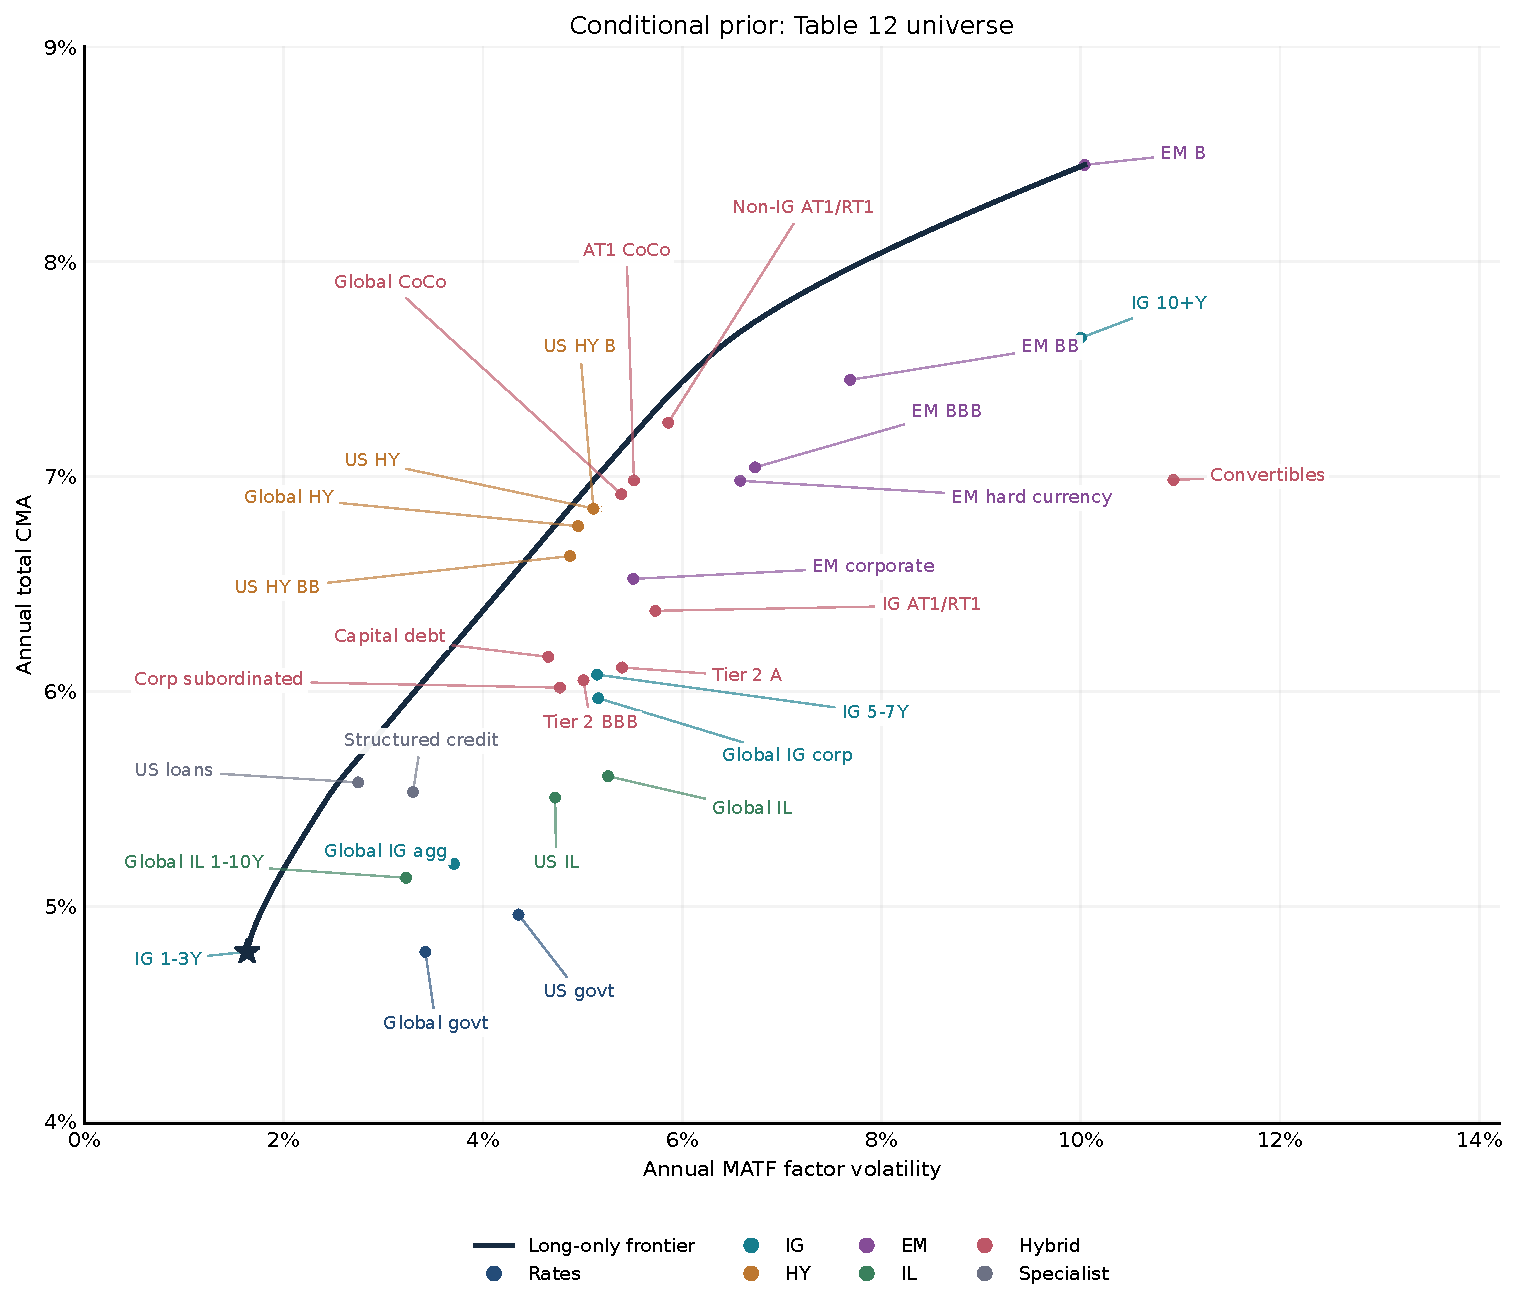
\includegraphics[width=.94\linewidth]{figures/fi_frontier.pdf}
\caption{Annual total CMA versus annual MATF factor volatility for the thirty Table 12 indices under Conditional prior. The curve is the fully invested, long-only efficient frontier; the star marks its minimum-variance endpoint. Labels use short names, with Bloomberg identifiers in Table 12. Residual risk is excluded. No expected-return forecasts are re-estimated for this exhibit.}
\end{figure}

\subsection{Clustering used by the estimator}

Figure 7 shows the response-clustering linkage returned by FactorLasso for the endpoint training sample, rather than clustering the fitted coefficients. The tree is common to Zero prior, Max-R2 prior, Expert prior and Conditional prior at this date. The configured cutoff fraction is 0.60 of the maximum pairwise distance, giving an actual distance cut of 0.6484 and three groups with 6, 19 and 5 members. The six-member group contains the government controls, Global IG agg and the three IL indices. The five-member group contains four CoCo/AT1 indices and US loans. The remaining nineteen form the third group. These groups describe return co-movement and can cross mandate categories; they are not credit-rating classifications. Shared cluster penalties provide the channel through which a prior change for one asset can alter a neighbour's fit.

\begin{figure}[pos=htbp]
\centering
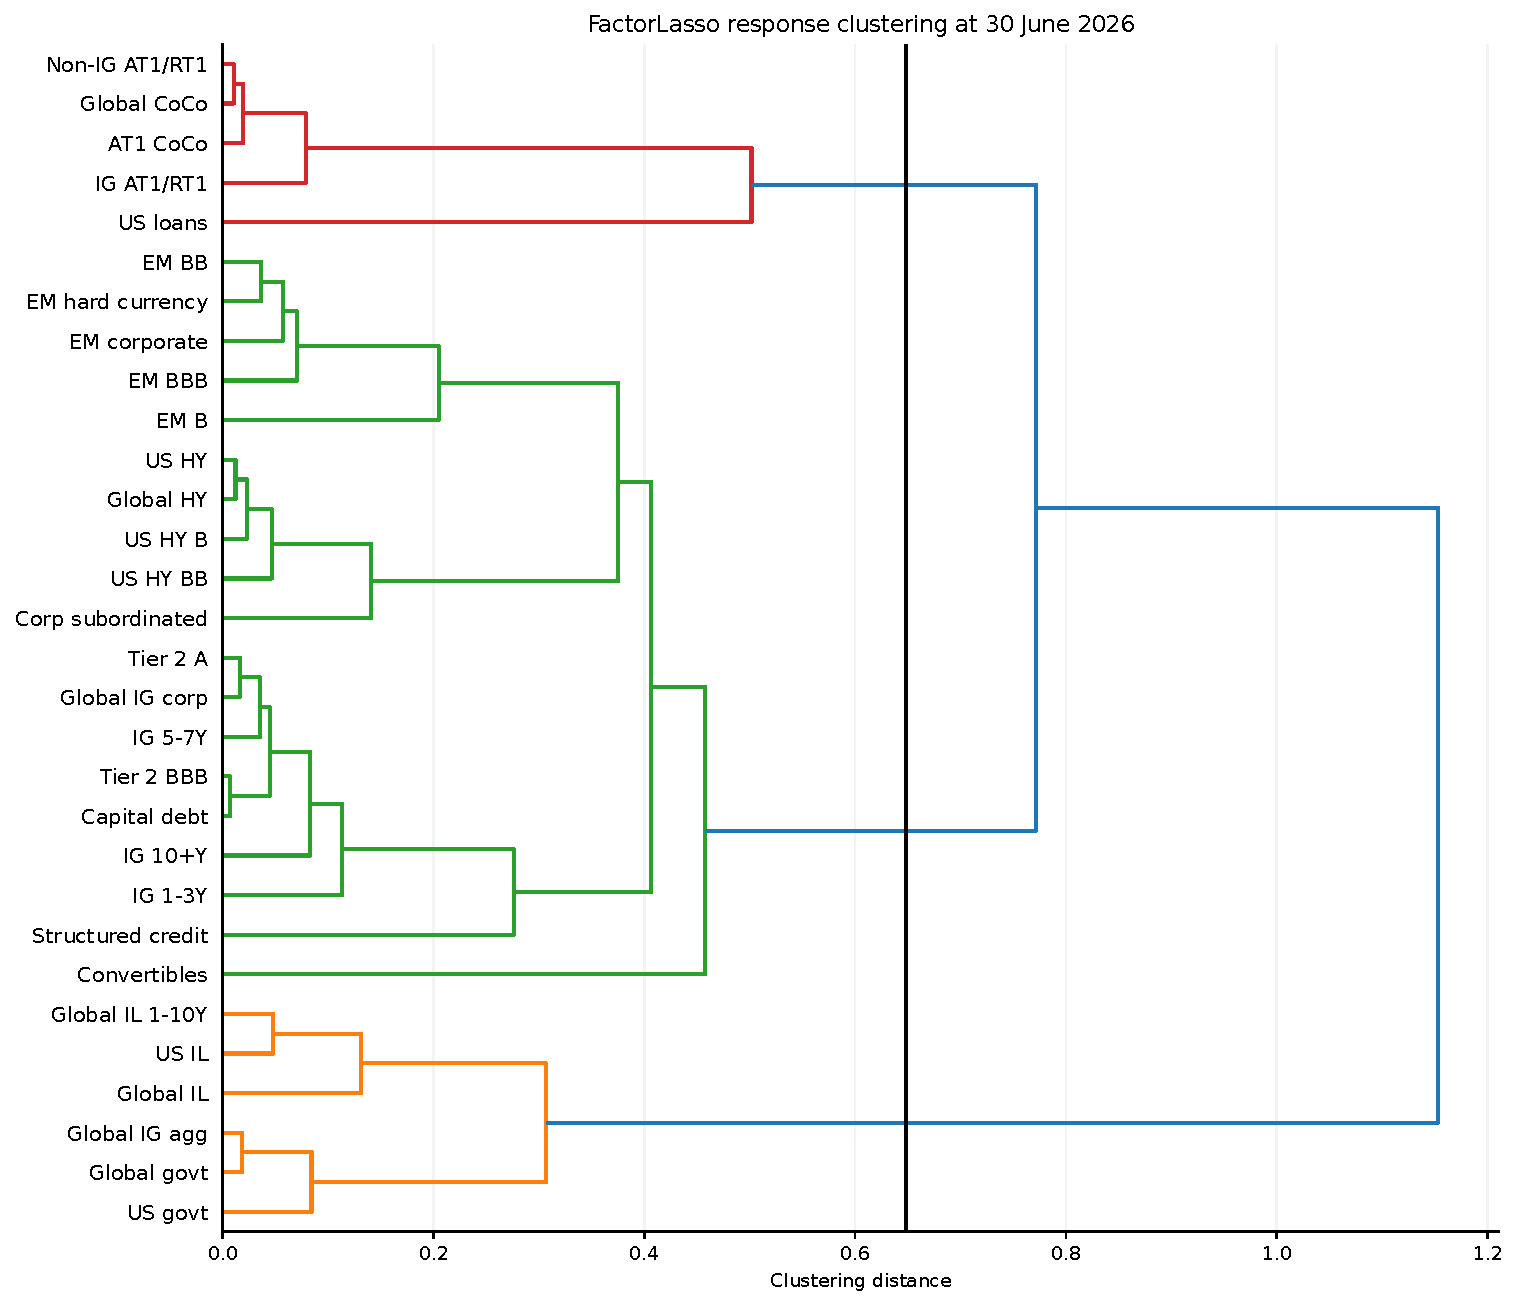
\includegraphics[width=.94\linewidth]{figures/fi_dendrogram.pdf}
\caption{The FactorLasso response dendrogram used by the thirty-index endpoint fits, rendered with QIS. The vertical line is the actual distance cut of 0.6484, corresponding to cutoff fraction 0.60; the three coloured groups match the saved endpoint cluster assignments. Leaf labels are the Table 12 short names. This endpoint tree is descriptive; held-out fits re-estimate clustering within each training sample.}
\end{figure}

\FloatBarrier\subsection{Historical stress scenarios}

We replay six one-month historical factor shocks through every endpoint model. Selection uses a fixed equal-weight reference basket of Global IG agg, Global HY and EM hard currency, over their 298 complete monthly observations from September 2001 to June 2026. The ranking statistic is the mean of their simple cash-relative returns, obtained from expm1 of monthly excess log returns. March 2020 is included explicitly; the five lowest other months are October 2008, September 2008, September 2022, June 2022 and June 2002. March 2020 ranks second, so the resulting set is also the reference basket's six worst months. This is a defined broad-bond ranking, not a claim that these months are worst for every instrument or risk factor. No fitted prior policy enters selection.

For asset $i$, policy $p$ and historical factor log-shock vector $f_s$, the displayed stress return is

\begin{equation}
R_{i,s}^{(p)}=100\left[\exp\left(\sum_k\widehat\beta_{i,k}^{(p)}f_{s,k}\right)-1\right].
\end{equation}

Negative numbers are percentage losses and positive numbers are gains. All twelve simultaneous factor shocks enter; Table 15 displays six principal factors for readability. Cash, intercept, residual alpha, regional expected-return overlays and residual shocks are excluded. Loadings are frozen at 30 June 2026 for all scenarios, including shocks before an instrument's inception. These are comparable current-exposure stress replays, not realised fund returns, forecasts available before the events, or held-out validation. Exact nonlinear valuation uses QIS and is independently checked with a scalar calculation.

\begin{table}[pos=htbp]
\centering
\small
\caption{Historical month selection and observed factor shocks. Reference is the equal-weight IG/HY/EM basket's simple cash-relative return; rank is from most negative to most positive over the 298 common months. Factor columns convert historical log shocks to simple percentage returns for display. The calculation uses the full twelve-factor log-shock vectors.}
\begin{adjustbox}{max width=\linewidth}
\begin{tabular}{lrrrrrrrr}
\toprule
Month & Reference \% & Rank & Rates \% & IG \% & HY \% & EM \% & Infl. \% & Equity \% \\
\midrule
Mar 2020 & -8.06 & 2 & +2.79 & -6.91 & -11.20 & -4.89 & -8.79 & -14.56 \\
Oct 2008 & -11.85 & 1 & -0.88 & -2.87 & -4.03 & -13.73 & -5.52 & -18.16 \\
Sep 2008 & -5.34 & 3 & -0.67 & -1.53 & -1.48 & -3.00 & -2.57 & -12.46 \\
Sep 2022 & -4.50 & 4 & -5.34 & -0.63 & -0.42 & -3.27 & -2.09 & -6.98 \\
Jun 2022 & -4.32 & 5 & -1.52 & -2.69 & -3.32 & -2.01 & -2.03 & -7.95 \\
Jun 2002 & -4.12 & 6 & +2.00 & -3.09 & -6.18 & -2.40 & -0.63 & -5.52 \\
\bottomrule
\end{tabular}
\end{adjustbox}
\end{table}

\begin{figure}[pos=htbp]
\centering
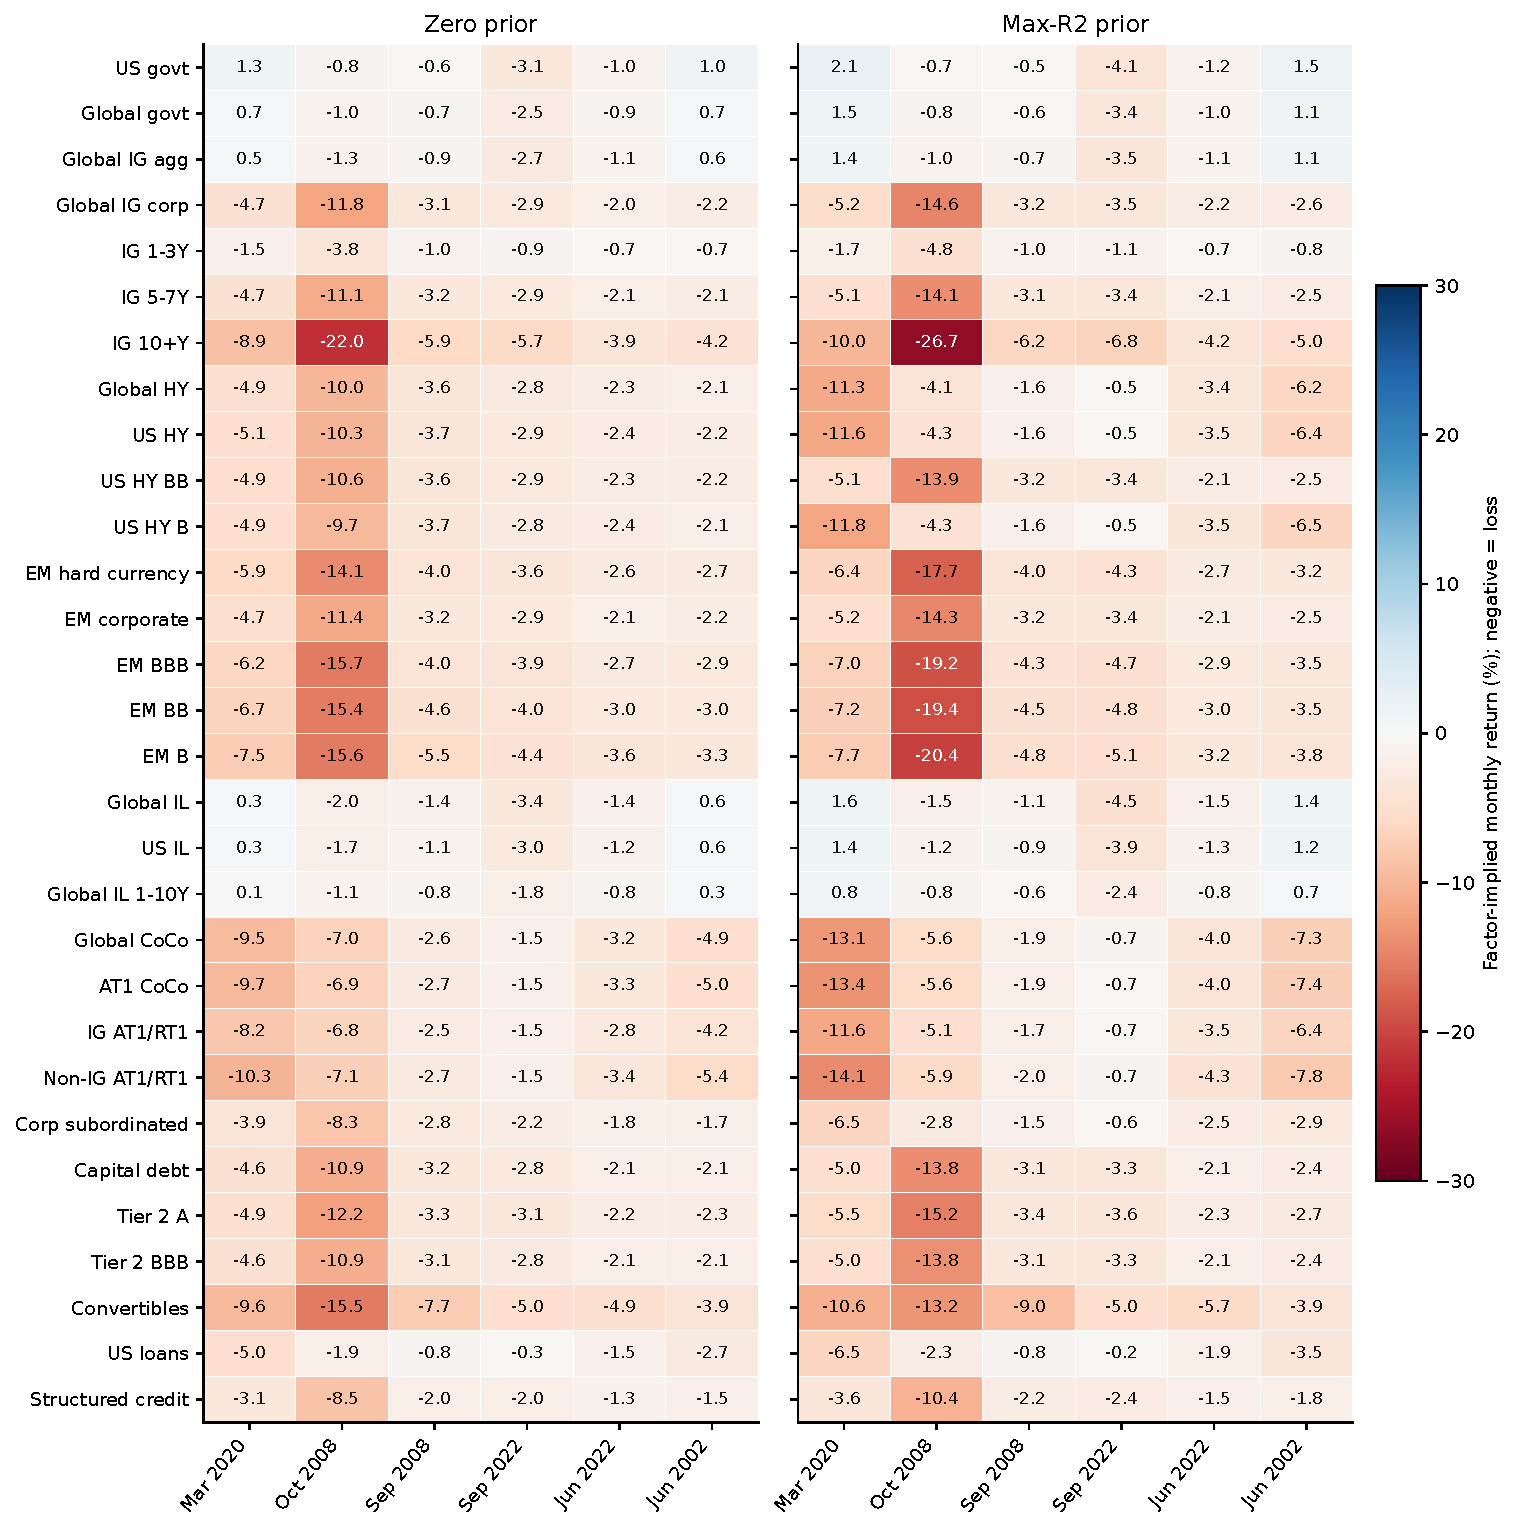
\includegraphics[width=.94\linewidth]{figures/fi_stress_indices_baseline.pdf}
\caption{Factor-implied stress returns for thirty indices under Zero prior and Max-R2 prior. Cells show percent returns to one decimal; red denotes loss, blue denotes gain and white is near zero. Figures 8-10 share the same symmetric scale. The month order follows Table 15, with March 2020 first.}
\end{figure}

\begin{figure}[pos=htbp]
\centering
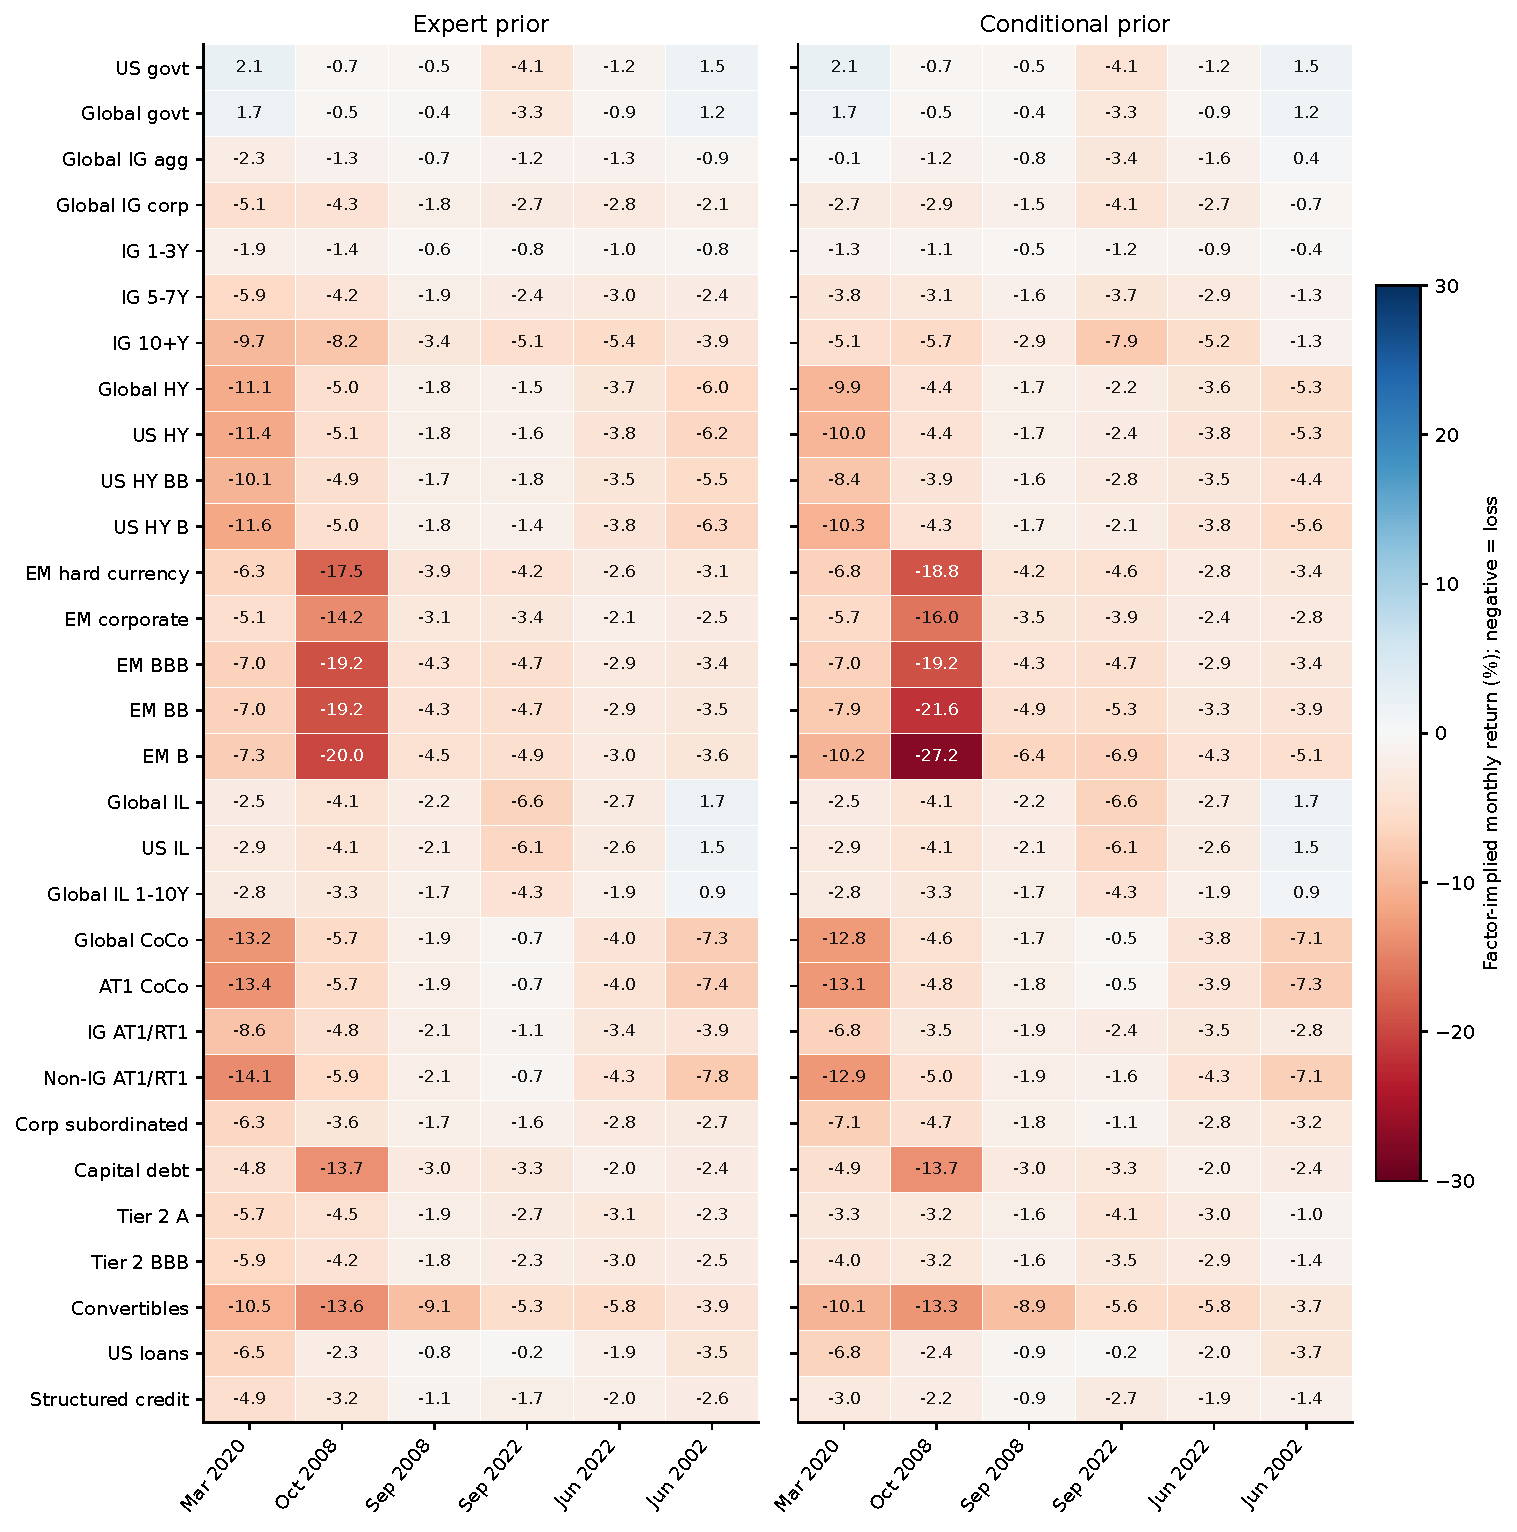
\includegraphics[width=.94\linewidth]{figures/fi_stress_indices_expert.pdf}
\caption{The same thirty-index stress replay under Expert prior and Conditional prior. Asset order, six historical shocks and colour scale match Figure 8, so differences arise only from the estimated endpoint loadings.}
\end{figure}

For Global IL in March 2020, Max-R2 prior versus Conditional prior implies +1.58\% versus -2.48\%; for Global IG agg the same comparison is +1.38\% versus -0.07\%, and for Global HY it is -11.27\% versus -9.86\%. The conditional Inflation loading changes the protection inferred from Rates alone. Expert conditioning need not make every estimated stress loss larger. The comparison measures sensitivity of current risk attribution to the prior choice; larger losses do not by themselves validate a model.

\begin{figure}[pos=htbp]
\centering
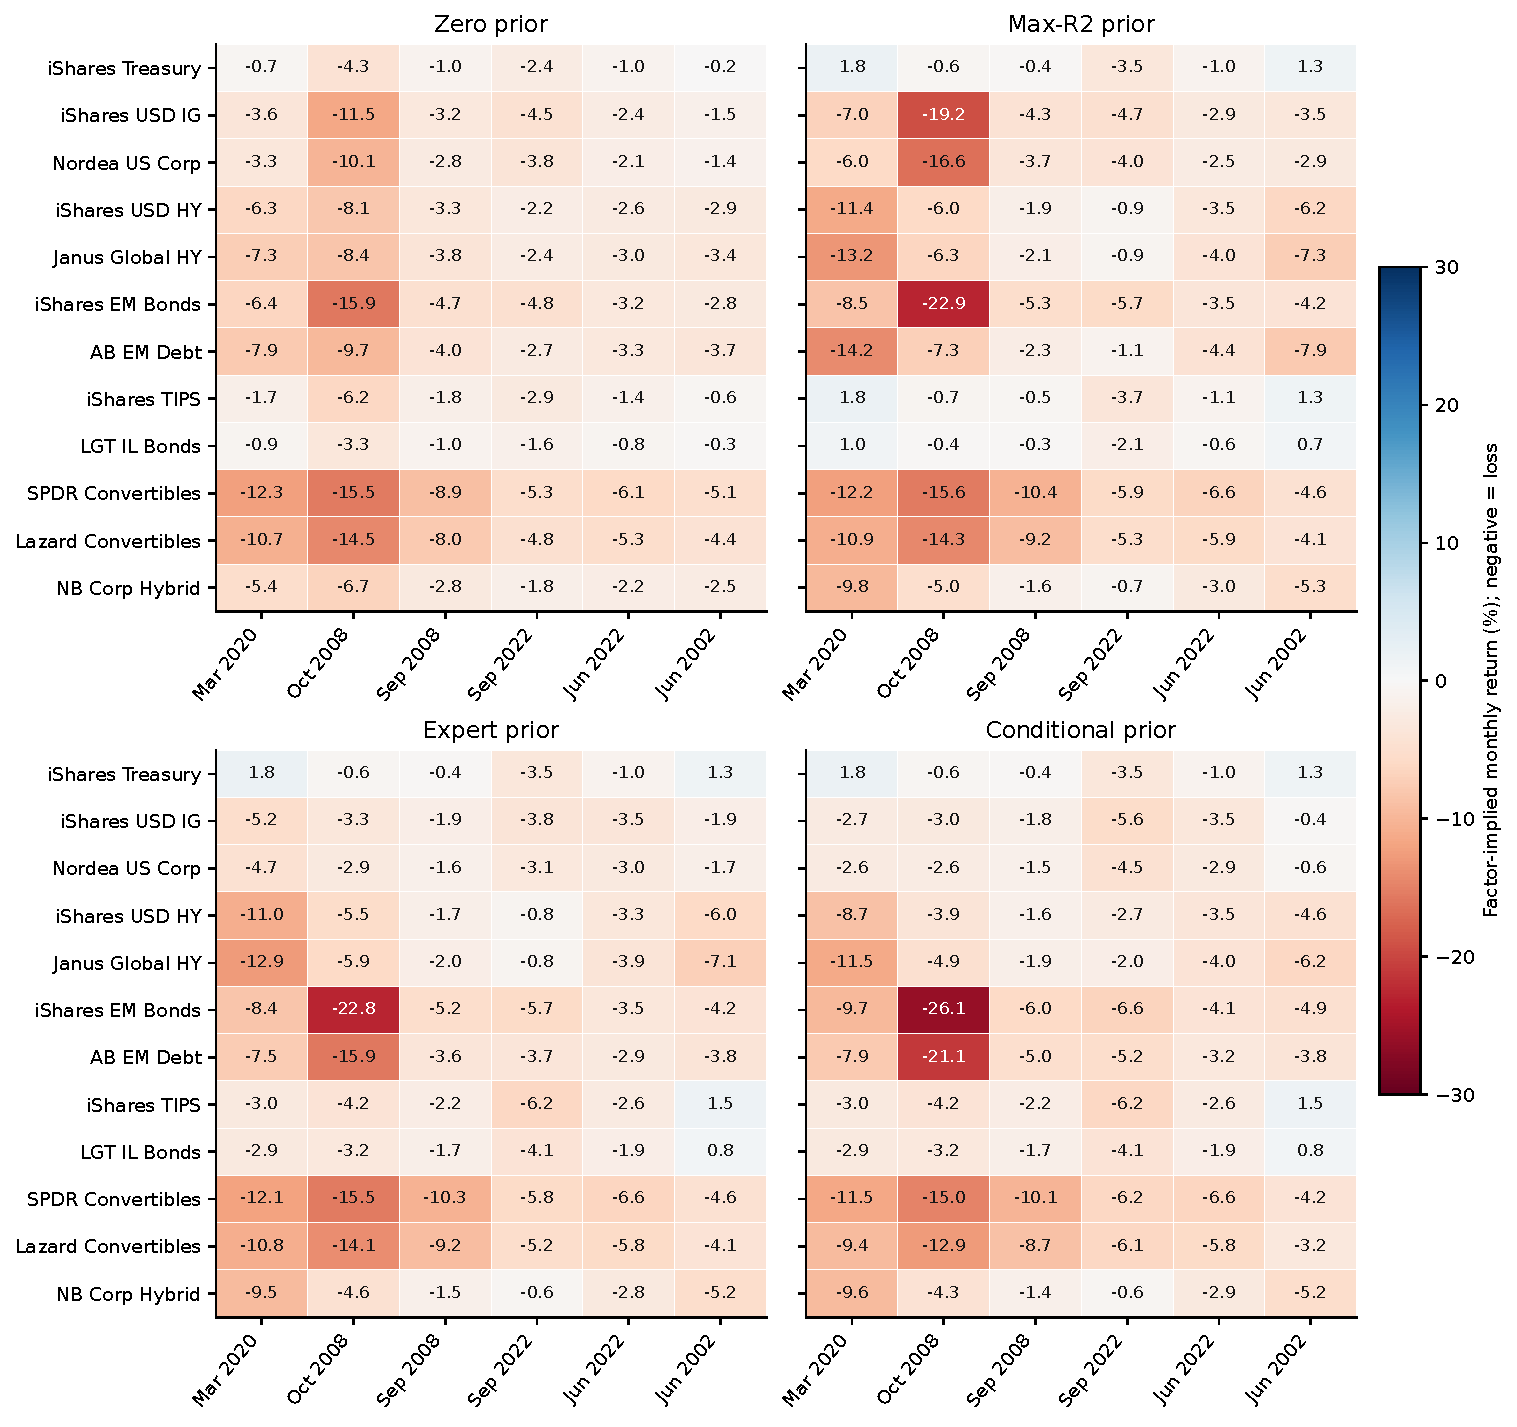
\includegraphics[width=.94\linewidth]{figures/fi_stress_funds.pdf}
\caption{The same six historical factor shocks applied to the twelve funds' endpoint loadings, using the same return convention and colour scale as Figures 8 and 9. Figures describe systematic exposure only; omitted residual and liquidity effects can materially change an investable vehicle's realised loss.}
\end{figure}

\FloatBarrier\section{Appendix: Sign-step revision and penalty controls}

Sign detection uses the original observation masks. Pre-inception rows and missing factor observations carry no sign information. The slope, adaptive weights and fit use the same native EWMA horizon. The gate sums response scores within each date before squaring, thereby retaining contemporaneous covariance among overlapping indices. Duplicating all responses in a pool leaves this statistic unchanged. The score variance assumes independent dates and is not a HAC estimator or an exact Student t test. A fixed span has bounded effective sample size, so a longer stored history alone cannot imply consistency.

Let $v_{tkj}$ mark valid observations and $w_t$ be the original-grid decay. For each pooled factor, $D_j=\sum_{t,k}w_tv_{tkj}x_{tj}^2$ and $\hat b_j=D_j^{-1}\sum_{t,k}w_tv_{tkj}x_{tj}y_{tk}$. The date score is $u_{tj}=w_tx_{tj}\sum_kv_{tkj}(y_{tk}-\hat b_jx_{tj})$. We use $\sum_tu_{tj}^2/D_j^2$, multiplied by $n_{\mathrm{eff},j}/(n_{\mathrm{eff},j}-1)$, where the effective count is based on valid weighted dates, not response cells. Fewer than two effective dates cannot pass a positive gate. The finite-sample multiplier is a screening convention.

The ablation retains observations, target regressions, current premiums, hard restrictions, cluster labels, per-response loss normalization and the calibrated penalty. It restores the old sign-input procedure and changes one sign component at a time. This is a controlled sign comparison at the current calibration, not an exact replay of the archived software stack. The final endpoint reproduces the refreshed main estimates. Rediscovering clusters gives the same partition and endpoint fits.

\begin{table}[pos=htbp]
\centering
\small
\caption{Conditional-prior sign-step ablation against the old sign-input procedure at the current calibration. Sign and block counts refer to endpoint cells; CMA changes are the largest absolute annual beta-times-premium change in each panel. RMSE uses identical held-out asset-month observations at span 60.}
\begin{adjustbox}{max width=\linewidth}
\begin{tabular}{lrrrrrr}
\toprule
Panel & Revision & Raw signs & Final signs & Blocks & Max CMA delta, bp & RMSE, \% \\
\midrule
Indices & Valid observations only & 0 & 0 & 12 & 80.1 & 1.349 \\
Indices & Valid observations + EWMA & 86 & 25 & 19 & 87.1 & 1.340 \\
Indices & EWMA + date-score gate & 115 & 49 & 23 & 110.4 & 1.340 \\
Funds & Valid observations only & 0 & 0 & 8 & 19.5 & 1.484 \\
Funds & Valid observations + EWMA & 30 & 10 & 13 & 27.4 & 1.479 \\
Funds & EWMA + date-score gate & 48 & 22 & 17 & 21.6 & 1.478 \\
\bottomrule
\end{tabular}
\end{adjustbox}
\end{table}

The mask-only repair can change coefficients without changing signs, because it changes adaptive penalty magnitudes. The dependence correction need not improve prediction at every threshold; its purpose is to prevent repeated response information from inflating the gate. Across all four policies, the combined revision improves held-out RMSE relative to the archived procedure in this fixed sample.

\begin{figure}[pos=htbp]
\centering
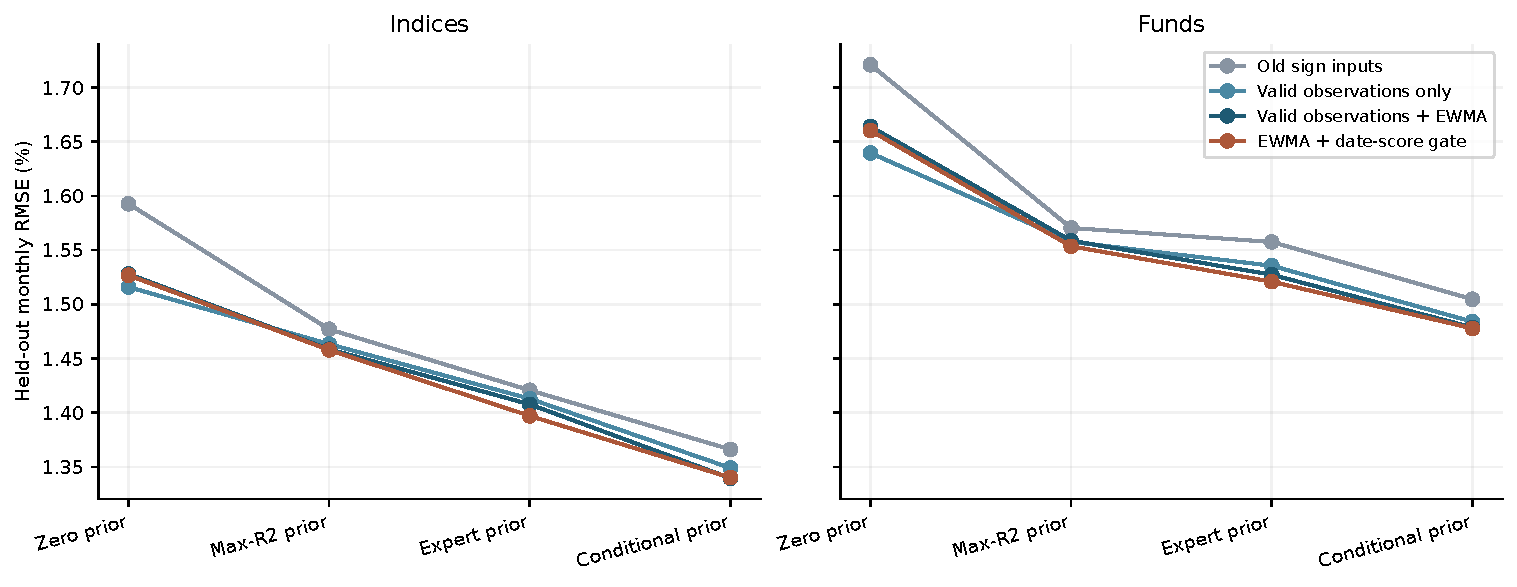
\includegraphics[width=.94\linewidth]{figures/fi_sign_revision.pdf}
\caption{Held-out monthly RMSE for the four complete policies at span 60. The same observations and factor vintage are used in every revision. Lower is better; these are return-reconstruction errors, not errors in long-term expected-return forecasts.}
\end{figure}

\begin{table}[pos=htbp]
\centering
\small
\caption{Matched prediction controls at span 60. Target-only uses the estimated target projected onto the same hard/solver sign set. Zero penalty uses the Conditional prior's feasible sign set with lambda zero. Every prediction uses the same weighted raw-residual intercept convention.}
\begin{adjustbox}{max width=\linewidth}
\begin{tabular}{lrrrr}
\toprule
Panel & Prior policy & FCGL, \% & Target only, \% & Zero penalty, \% \\
\midrule
Indices & Max-R2 prior & 1.458 & 1.550 & -- \\
Indices & Expert prior & 1.397 & 1.559 & -- \\
Indices & Conditional prior & 1.340 & 1.409 & 1.334 \\
Funds & Max-R2 prior & 1.553 & 1.715 & -- \\
Funds & Expert prior & 1.521 & 1.669 & -- \\
Funds & Conditional prior & 1.478 & 1.518 & 1.437 \\
\bottomrule
\end{tabular}
\end{adjustbox}
\end{table}

\FloatBarrier
The fitted policy improves on its target-only counterpart, so it is not merely the target returned unchanged. However, the sign-constrained zero-penalty model performs slightly better for both indices and funds at the current fixed calibration. This limits any claim that the specified penalty is universally beneficial. At the endpoint many coefficients still sit on their targets: this is prior-centred shrinkage, and the quality of the target rule remains central to the result.

All sign variants use the same per-response valid-weight normalization and fixed calibrated penalty described in Section 2.3. The comparison isolates sign mechanics; changes from the earlier draft also include the separately approved credit premium calibration. Neither premiums nor the penalty are selected from these sign outcomes.

\FloatBarrier\clearpage\section*{Computational provenance and availability}

The editorial source is manuscript.md; article.tex is generated through the existing CAS build. The source manifest identifies the frozen roster, input hashes, policy protocol and all stage receipts. Numerical tables are regenerated before compilation, and deliberately corrupted tables must be rejected by the same verifier. The source bundle includes the research orchestration and two offline examples. Licensed return histories and original workbooks remain local and are not included in the companion bundle.

Estimation belongs to \href{https://github.com/ArturSepp/FactorLasso}{FactorLasso} (\href{https://github.com/ArturSepp/FactorLasso/blob/main/CITATION.cff}{citation}). Private universe preparation and CMA arithmetic use the existing Rosaa owners; risk integration uses \href{https://github.com/ArturSepp/OptimalPortfolios}{OptimalPortfolios}. Return handling, dependent resampling and scientific rendering use \href{https://github.com/ArturSepp/QuantInvestStrats}{QIS} (\href{https://github.com/ArturSepp/QuantInvestStrats/blob/main/CITATION.cff}{citation}). No private runtime dependency is added to the public FactorLasso package.
\FloatBarrier
\begingroup
\setstretch{1}
\bibliographystyle{cas-model2-names}
\bibliography{refs}
\endgroup
\end{document}
